\documentclass[11pt,a4paper]{article}

% --- Packages ---
\usepackage[utf8]{inputenc}
\usepackage[T1]{fontenc}
\usepackage{amsmath,amssymb,amsfonts}
\usepackage{graphicx}
\usepackage{booktabs}
\usepackage{hyperref}
\usepackage{natbib}
\usepackage[margin=1in]{geometry}
\usepackage{algorithm}
\usepackage{algorithmic}
\usepackage{multirow}
\usepackage{caption}
\usepackage{subcaption}
\usepackage{xcolor}
\usepackage{float}

% --- Hyperref setup ---
\hypersetup{
    colorlinks=true,
    linkcolor=blue,
    citecolor=blue,
    urlcolor=blue
}

% --- Custom commands ---
\newcommand{\R}{\mathbb{R}}
\newcommand{\E}{\mathbb{E}}
\newcommand{\Prob}{\mathbb{P}}

\title{Continuous Gaussian Hidden Markov Models for Equity and Volatility Index Dynamics:\\A Baum-Welch Approach Without Jump Augmentation}

\author{
    Abdulrahman Alswaidan\thanks{Cornell University, Robert Frederick Smith School of Chemical and Biomolecular Engineering, Ithaca, NY, USA.}
    \and
    Jeffrey D.\ Varner\thanks{Cornell University, Robert Frederick Smith School of Chemical and Biomolecular Engineering, Ithaca, NY, USA. Email: \texttt{jdv27@cornell.edu}.}
}

\date{\today}

\begin{document}

\maketitle

% ========================================================================================= %
\begin{abstract}
We present a continuous hidden Markov model (CHMM) with Gaussian emissions trained via the Baum-Welch (Expectation-Maximization) algorithm for generating synthetic financial time series that preserve the canonical stylized facts of asset returns.
Unlike the discrete-state framework of \citet{alswaidan2026hybrid}, which requires Laplace quantile binning and a Poisson jump-duration mechanism to achieve volatility clustering, we show that the continuous model at moderate state resolution ($K = 6$--$13$) reproduces all three stylized facts---heavy-tailed distributions, negligible linear autocorrelation, and persistent volatility clustering---without jump augmentation, thereby eliminating two tunable hyperparameters ($\epsilon$, $\lambda$) and the discretization step entirely.

We benchmark the CHMM against five alternative generators on ten years of daily S\&P~500 ETF (SPY) data: bootstrap resampling, Gaussian and Laplace i.i.d.\ generators, GARCH(1,1), and the discrete HMM with jumps from \citet{alswaidan2026hybrid}.
Evaluation uses seven complementary metrics---Kolmogorov--Smirnov and Anderson--Darling pass rates, excess kurtosis, autocorrelation function mean absolute error (ACF-MAE), Wasserstein-1 and Hellinger distances, and quantile coverage---applied to 1,000 simulated paths in both in-sample (2014--2024) and out-of-sample (2025) windows.
Cross-asset generalization to NVDA, JNJ, and JPM confirms adaptability to diverse risk profiles.

We further extend the framework to CBOE Volatility Index (VIX) and VXX log returns, demonstrating that the CHMM captures the distinct statistical properties of volatility indices---including stronger mean reversion, positive skewness, and pronounced regime structure.
The VIX regime decomposition provides a natural bridge to option pricing: median VIX levels per decoded regime define a volatility map that drives regime-switching geometric Brownian motion paths, producing implied volatility surfaces that we compare against the Heston stochastic volatility benchmark.

\bigskip\noindent
\textbf{Keywords:} Continuous Hidden Markov Model, Baum-Welch Algorithm, Stylized Facts, Volatility Clustering, Regime-Switching, Synthetic Financial Data, VIX, Option Pricing
\end{abstract}

% ========================================================================================= %
\section{Introduction}
\label{sec:introduction}
Generating synthetic financial time series that faithfully preserve the statistical properties of real market data is a central challenge in quantitative finance.
High-fidelity synthetic data are essential for stress testing risk models against plausible but unobserved market scenarios, validating portfolio optimization algorithms, and augmenting limited training sets for machine learning pipelines \citep{assefa2020generating, jordon2022synthetic}.
Empirical equity excess growth rates exhibit three well-documented statistical regularities---heavy-tailed (leptokurtic) distributions, negligible linear autocorrelation in raw returns, and persistent volatility clustering---that any generative framework must simultaneously reproduce to be considered statistically faithful \citep{cont2001empirical, mandelbrot1963variation}.

Parametric approaches to synthetic data generation face a fundamental tension between distributional accuracy and temporal fidelity.
GARCH models \citep{engle1982autoregressive, bollerslev1986generalized} excel at reproducing the slow decay of the autocorrelation function (ACF) of absolute returns---the hallmark of volatility clustering---but their unimodal innovation distribution cannot represent the multi-regime structure of equity markets, leading to poor distributional fit.
Conversely, i.i.d.\ generators that match the marginal distribution (e.g., Laplace sampling) achieve high distributional pass rates but produce flat ACF profiles by construction.
Hidden Markov models (HMMs) offer a middle path: the latent regime structure can simultaneously generate heavy-tailed mixtures and temporal persistence through the transition dynamics.

However, the application of HMMs to financial stylized facts has been constrained by an influential negative result.
\citet{ryden1998stylized} systematically evaluated Gaussian-emission HMMs with $K = 2$--$3$ states against the canonical stylized facts and concluded that while HMMs reproduce heavy tails and negligible return autocorrelation, they \emph{fail} to capture the slow decay of the ACF of absolute returns.
The mechanism is clear: with few states, the geometric sojourn-time distribution of a standard Markov chain produces exponentially fast ACF decay, insufficient to match the hyperbolic-like persistence observed empirically.
\citet{bulla2006stylized} subsequently showed that hidden semi-Markov models (HSMMs), which replace the geometric sojourn distribution with flexible alternatives, restore ACF fidelity---but at the cost of substantially increased model complexity.

\citet{alswaidan2026hybrid} proposed an alternative solution within the discrete HMM framework: a Poisson jump-duration mechanism that forces the model to dwell in tail states for empirically calibrated durations.
That approach achieved 91--95\% Kolmogorov--Smirnov (KS) pass rates across 424 US equities and partially reproduced volatility clustering.
However, the discrete framework introduced three sources of complexity: (i)~Laplace quantile binning, which discretizes continuous observations and introduces quantization error; (ii)~two additional hyperparameters ($\epsilon$ for jump probability and $\lambda$ for mean jump duration) requiring grid search calibration; and (iii)~within-bin Student-$t$ emission models whose parameters are estimated separately from the transition structure.

In this paper, we show that these complexities are unnecessary.
A continuous Gaussian HMM (CHMM) trained via the Baum-Welch algorithm \citep{baum1970maximization, rabiner1986introduction} with quantile-based initialization reproduces all three canonical stylized facts at moderate state resolution ($K = 6$--$13$) \emph{without} requiring jump augmentation, discretization, or separate emission fitting.
The key insight is that the negative result of \citet{ryden1998stylized} is an artifact of insufficient state resolution: at $K \geq 3$ with proper initialization, the Baum-Welch algorithm learns a transition matrix with sufficient diagonal dominance in high-volatility states to generate slow ACF decay, effectively approximating the flexible sojourn-time distributions of HSMMs through a mixture of geometric distributions.

The contributions of this work are:
\begin{enumerate}
    \item \textbf{Baum-Welch training without jump augmentation.}
    We train continuous Gaussian emission parameters $(\mu_k, \sigma_k)$ and the transition matrix $\mathbf{T}$ jointly from raw observations via the Baum-Welch algorithm with quantile-based initialization.
    The resulting CHMM achieves 90--94\% KS pass rates and ACF-MAE of 0.046--0.049 on absolute returns---comparable to GARCH(1,1) (ACF-MAE $= 0.047$)---without any jump mechanism, eliminating two hyperparameters ($\epsilon$, $\lambda$) and the discretization step.

    \item \textbf{Contradiction of the Ryd\'{e}n et al.\ (1998) consensus.}
    We demonstrate that the widely cited limitation of Gaussian HMMs---inability to reproduce volatility clustering---is a consequence of testing only $K = 2$--$3$ states.
    At moderate $K$, the learned transition matrix develops sufficient persistence in high-volatility states to achieve ACF-MAE comparable to GARCH, which we show is effectively an approximation to the HSMM solution of \citet{bulla2006stylized}.

    \item \textbf{Comprehensive five-model benchmark.}
    We evaluate the CHMM against bootstrap resampling, Gaussian and Laplace i.i.d.\ generators, and GARCH(1,1) using seven complementary metrics---KS and Anderson--Darling (AD) pass rates, excess kurtosis, ACF-MAE, Wasserstein-1 and Hellinger distances, and quantile coverage---on 1,000 simulated paths in both in-sample (2014--2024) and out-of-sample (2025) windows.

    \item \textbf{State resolution analysis.}
    We systematically vary $K \in \{3, 6, 9, 11, 13\}$ and show that distributional fidelity improves with $K$ while ACF-MAE remains remarkably stable, and quantile coverage is 100\% at all resolutions.

    \item \textbf{Cross-asset and volatility index generalization.}
    We confirm robustness across NVDA, JNJ, and JPM (97--100\% IS KS), and extend the framework to CBOE VIX and VXX log returns, demonstrating that the CHMM captures the distinct statistical properties of volatility indices and provides a natural bridge to regime-switching option pricing.
\end{enumerate}

The remainder of this paper is organized as follows.
Section~\ref{sec:related} reviews the relevant literature on stylized facts, parametric models, HMMs, and deep generative approaches.
Section~\ref{sec:methods} describes the data, the CHMM specification, the Baum-Welch training procedure, the benchmark models, and the validation metrics.
Section~\ref{sec:results} presents the empirical results: descriptive statistics, five-model comparison, state resolution sensitivity, out-of-sample evaluation, cross-asset generalization, and the VIX/VXX extension.
Section~\ref{sec:discussion} interprets the findings---particularly the ACF-MAE result and its implications for the Ryd\'{e}n et al.\ consensus---and identifies limitations.
Section~\ref{sec:conclusion} summarizes the contributions and outlines future directions.


\section{Related Work}
\label{sec:related}
\input{sections/related_v2}

\section{Methods}
\label{sec:methods}
\input{sections/methods_v2}

\section{Empirical Study}
\label{sec:results}
\subsection{Descriptive Statistics and Stylized Facts}
\label{sec:descriptive}

Descriptive statistics confirmed that all three canonical stylized facts were present in both the in-sample (2014--2024, $T = 2{,}766$) and out-of-sample (2025, $T = 219$) windows (Table~\ref{tab:descriptive}).
The in-sample excess growth rates exhibited excess kurtosis of 7.707, strong negative skewness ($-0.753$), and a Jarque--Bera statistic of 7107.4, decisively rejecting the null hypothesis of normality ($p < 0.001$).
The Ljung--Box test on absolute returns rejected the null of no autocorrelation ($\text{LB} = 3057.9$, $p < 0.001$), confirming pronounced volatility clustering.
The Ljung--Box test on raw returns also rejected ($\text{LB} = 145.3$), reflecting mild serial dependence in the level series.

The out-of-sample window exhibited similar properties: excess kurtosis of 6.242, stronger negative skewness ($-1.071$), and a Jarque--Bera statistic of 397.4.
Notably, the Ljung--Box test on raw OoS returns failed to reject ($\text{LB} = 28.1$), consistent with efficient pricing in the shorter sample, while the test on absolute returns strongly rejected ($\text{LB} = 150.4$), confirming that volatility clustering persisted in the test period.
These properties are visualized in Figure~\ref{fig:stylized_facts}.

\begin{table}[t]
\centering
\caption{Descriptive statistics and stylized-fact tests for SPY daily excess growth rates. IS: 2014--2024 ($T = 2{,}766$); OoS: 2025 ($T = 219$). JB = Jarque--Bera normality test. LB = Ljung--Box autocorrelation test at lag~20. $^*$~denotes rejection at $\alpha = 0.05$.}
\label{tab:descriptive}
\begin{tabular}{lcc}
\toprule
Statistic & IS Observed & OoS Observed \\
\midrule
Mean (annualized) & 0.11 & 0.13 \\
Std Dev (annualized) & 2.14 & 2.31 \\
Skewness & $-0.753$ & $-1.071$ \\
Excess Kurtosis & 7.707 & 6.242 \\
JB test statistic & 7107.4 & 397.4 \\
JB decision & reject$^*$ ($p < 0.001$) & reject$^*$ ($p < 0.001$) \\
LB test on $G_t$ (lag 20) & reject$^*$ (145.3) & fail to reject (28.1) \\
LB test on $|G_t|$ (lag 20) & reject$^*$ (3057.9) & reject$^*$ (150.4) \\
\bottomrule
\end{tabular}
\end{table}

\begin{figure}[t]
\centering

\includegraphics[width=\textwidth]{sections/figs/Fig-1-Stylized-Facts.pdf}
\caption{Empirical stylized facts of SPY daily excess growth rates (2014--2024). Panel~(a): leptokurtic marginal distribution with Gaussian and Laplace fits. Panel~(b): normal Q-Q plot confirming heavy tails. Panel~(c): near-zero autocorrelation of raw returns. Panel~(d): persistent autocorrelation of absolute returns characterizing volatility clustering.}
\label{fig:stylized_facts}
\end{figure}

\subsection{Baum-Welch Training and Model Internals}
\label{sec:model_internals}

We trained continuous Gaussian HMMs for $K \in \{3, 6, 9, 11, 13\}$ states using the Baum-Welch algorithm with $\texttt{max\_iter} = 60$.
All models converged within the iteration budget, with log-likelihood plateauing after 20--40 iterations (Figure~\ref{fig:convergence_all}, Appendix~\ref{sec:supplemental}).

Figure~\ref{fig:model_internals} shows the fitted model internals for $K = 13$: the learned emission distributions span the full range of observed returns, with tail states capturing extreme crash and boom regimes.
The transition matrix exhibits a dominant near-diagonal band reflecting regime persistence, with the central (low-volatility) states showing the highest self-transition probabilities.
Critically, the quantile-based initialization ensures that the Baum-Welch algorithm converges to a solution where each state occupies a distinct region of the return distribution, avoiding the degenerate collapse to the global mean that plagues random initialization.

\begin{figure}[t]
\centering
\begin{subfigure}[b]{0.48\textwidth}
    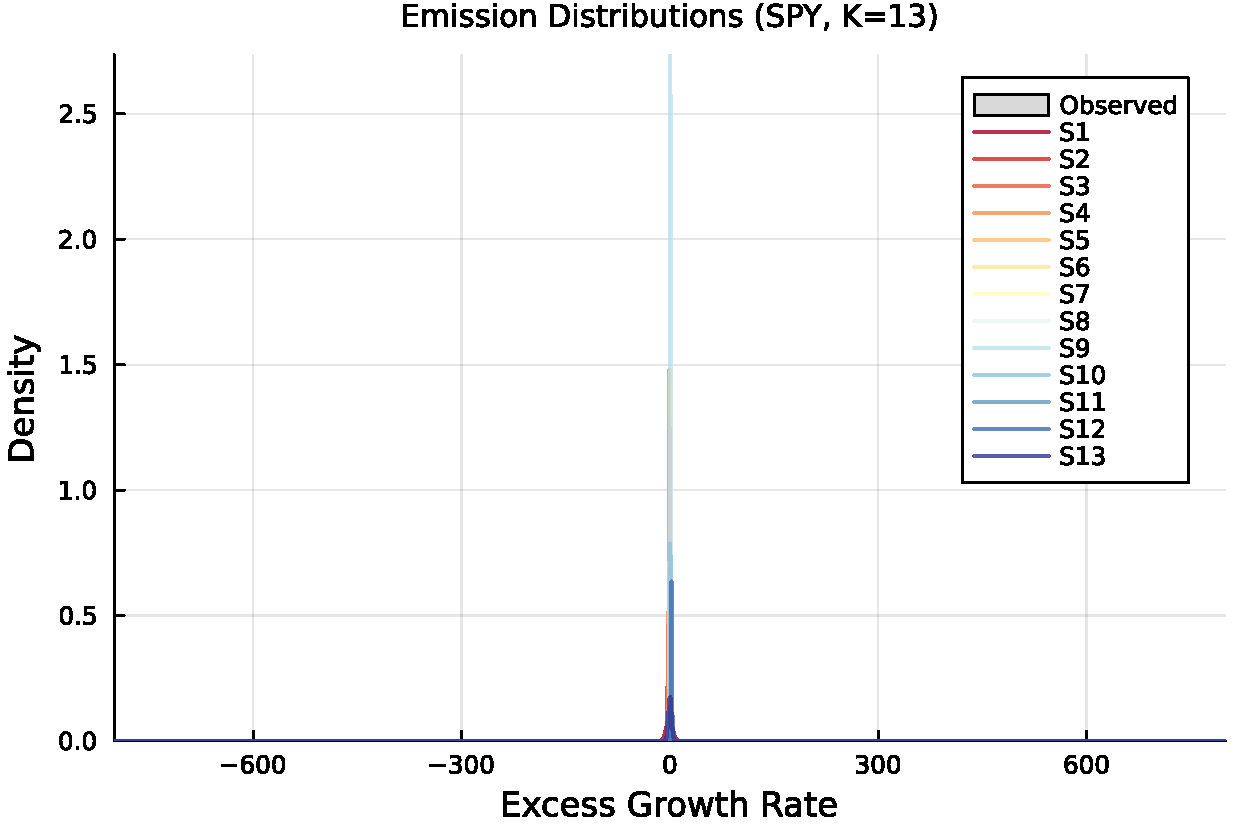
\includegraphics[width=\textwidth]{sections/figs/Fig-Emission-PDFs-K13.pdf}
    \caption{Emission distributions ($K = 13$)}
\end{subfigure}
\hfill
\begin{subfigure}[b]{0.48\textwidth}
    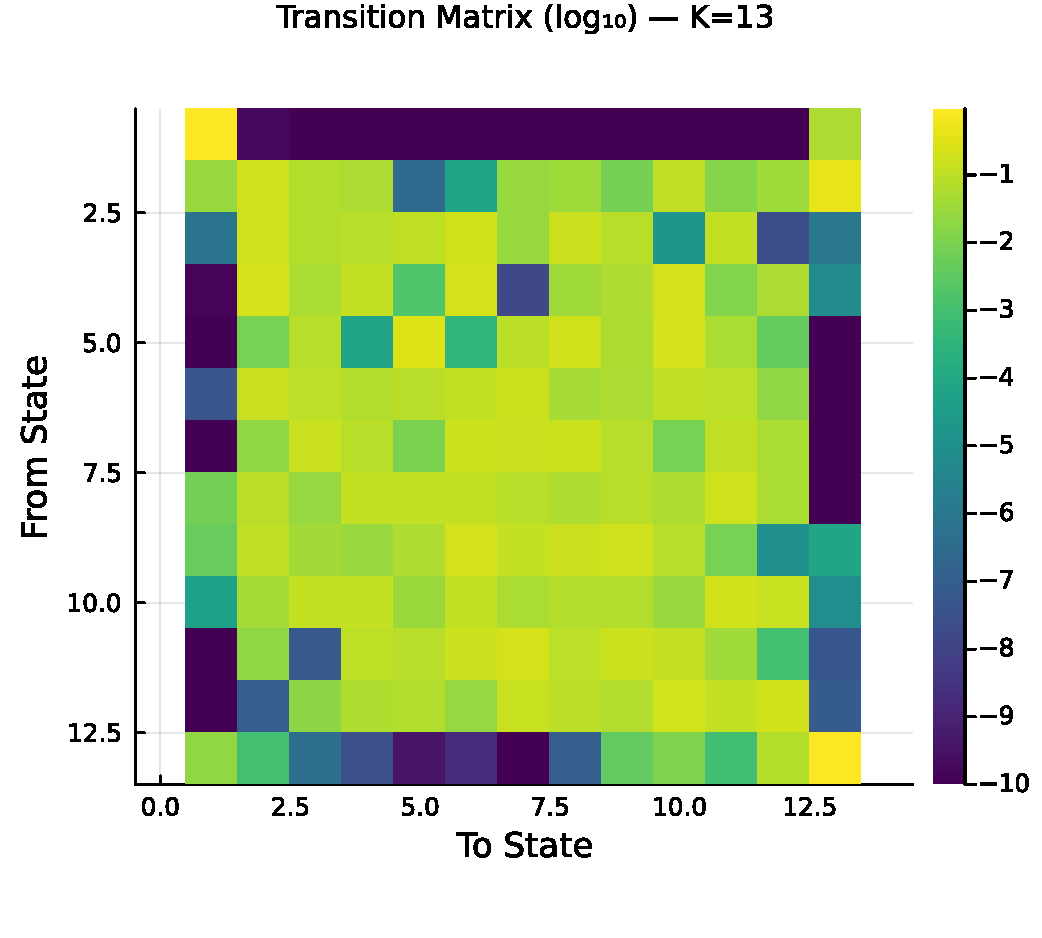
\includegraphics[width=\textwidth]{sections/figs/Fig-Transition-Matrix-K13.pdf}
    \caption{Transition matrix (log$_{10}$ scale)}
\end{subfigure}
\caption{Fitted model internals for SPY with $K = 13$ states. (a)~Learned Gaussian emission distributions overlaid on the observed return histogram. (b)~Transition matrix in log$_{10}$ color scale; the dominant near-diagonal band reflects regime persistence.}
\label{fig:model_internals}
\end{figure}

\subsection{Five-Model Comparison}
\label{sec:model_comparison}

Table~\ref{tab:model_comparison} and Figure~\ref{fig:is_comparison} present the in-sample and out-of-sample validation results for all five generators.
The CHMM results correspond to $K = 11$ (best IS KS); sensitivity to $K$ is analyzed in Section~\ref{sec:k_sensitivity}.

\paragraph{Bootstrap (Non-Parametric Ceiling).}
Bootstrap resampling achieved 99.9\% KS and 99.9\% AD pass rates in-sample, confirming it as the distributional ceiling.
It produced simulated kurtosis (7.44) closest to observed (7.71) and 100\% quantile coverage.
However, the bootstrap's ACF-MAE (0.0616) was the highest among all models except Laplace, reflecting the destruction of temporal structure by i.i.d.\ resampling.
The Wasserstein-1 (0.061) and Hellinger (0.048) distances were the lowest, as expected.

\paragraph{Gaussian i.i.d.\ (Negative Control).}
The Gaussian generator achieved 0\% KS and 0\% AD in-sample, confirming the categorical inadequacy of the normal distribution for financial returns.
Its simulated kurtosis was $-0.0$ (i.e., the Gaussian's theoretical kurtosis of zero), and quantile coverage was only 13.1\%.
The out-of-sample results were artificially inflated (74.0\% KS) due to the smaller OoS sample size ($T = 219$), which reduces the KS test's power to detect distributional differences.

\paragraph{Laplace i.i.d.}
The Laplace generator achieved 98.3\% KS and 97.0\% AD in-sample, demonstrating that the Laplace distribution provides a reasonable approximation to the marginal distribution of equity returns.
However, its simulated kurtosis (2.99) fell well short of the observed 7.71, and as an i.i.d.\ generator it produced flat ACF profiles (ACF-MAE $= 0.0616$, comparable to bootstrap).
The 76.8\% quantile coverage indicates that the Laplace distribution's fixed tail decay rate cannot fully envelop the observed quantile range.

\paragraph{GARCH(1,1).}
GARCH achieved the best ACF-MAE (0.0472) among all models, confirming its superior temporal fidelity.
However, it catastrophically failed the distributional tests: 13.0\% KS and 3.2\% AD in-sample.
The simulated kurtosis (6.3) was reasonably close to observed, but the Wasserstein-1 distance (0.245) and Hellinger distance (0.102) were substantially worse than the CHMM.
Quantile coverage was only 39.4\%.
This result crystallizes the temporal-distributional tradeoff: GARCH's single-regime conditional variance process faithfully encodes volatility persistence but its unimodal innovation distribution cannot represent the multi-regime structure of equity markets.

\paragraph{CHMM.}
The continuous HMM achieved 94.4\% KS and 85.3\% AD in-sample---competitive with the bootstrap (99.9\%) and Laplace (98.3\%) on KS, and substantially outperforming GARCH (13.0\%).
The ACF-MAE of 0.0475 was virtually identical to GARCH (0.0472), demonstrating that the CHMM reproduces volatility clustering \emph{without} a dedicated jump mechanism or conditional variance equation.
This is the central finding of this paper: the Ryd\'{e}n et al.\ limitation is resolved by moderate state resolution.

The Wasserstein-1 distance (0.11) and Hellinger distance (0.077) were comparable to the Laplace baseline and substantially better than GARCH.
Quantile coverage was 100\%, matching the bootstrap ceiling.
The simulated kurtosis (4.22) underestimated the observed 7.71, reflecting the Gaussian emission assumption's inability to produce power-law tails---a limitation we discuss in Section~\ref{sec:discussion}.

The out-of-sample results confirmed robust generalization: the CHMM achieved 93.8\% KS and 86.9\% AD on the held-out 2025 data, with minimal degradation from the in-sample performance.

\begin{table}[t]
\centering
\caption{Model comparison for SPY (1,000 simulated paths, $\alpha = 0.05$). IS: 2014--2024 ($T = 2{,}766$); OoS: 2025 ($T = 219$). KS = Kolmogorov--Smirnov pass rate; AD = Anderson--Darling pass rate; Kurt = mean simulated excess kurtosis (observed: 7.71); ACF-MAE = mean absolute error of $\text{ACF}(|G_t|)$ over 252 lags; $W_1$ = Wasserstein-1 distance; $H$ = Hellinger distance; Cov = quantile coverage (\%). $\uparrow$/$\downarrow$ indicate preferred direction.}
\label{tab:model_comparison}
\small
\begin{tabular}{l cc cc c c c c c}
\toprule
& \multicolumn{2}{c}{KS (\%) $\uparrow$} & \multicolumn{2}{c}{AD (\%) $\uparrow$} & & & & & \\
\cmidrule(lr){2-3} \cmidrule(lr){4-5}
Model & IS & OoS & IS & OoS & Kurt $\approx$ & ACF-MAE $\downarrow$ & $W_1$ $\downarrow$ & $H$ $\downarrow$ & Cov (\%) $\uparrow$ \\
\midrule
\textit{Observed} & --- & --- & --- & --- & 7.71 & --- & --- & --- & --- \\
Bootstrap & 99.9 & 98.6 & 99.9 & 99.2 & 7.44 & 0.0616 & 0.061 & 0.0478 & 100.0 \\
Gaussian & 0.0 & 74.0 & 0.0 & 75.6 & $-0.0$ & 0.0615 & 0.399 & 0.1513 & 13.1 \\
Laplace & 98.3 & 97.7 & 97.0 & 99.1 & 2.99 & 0.0616 & 0.120 & 0.0786 & 76.8 \\
GARCH(1,1) & 13.0 & 87.3 & 3.2 & 83.2 & 6.30 & 0.0472 & 0.245 & 0.1019 & 39.4 \\
CHMM & 94.4 & 93.8 & 85.3 & 86.9 & 4.22 & 0.0475 & 0.110 & 0.0772 & 100.0 \\
\bottomrule
\end{tabular}
\end{table}

\begin{figure}[t]
\centering
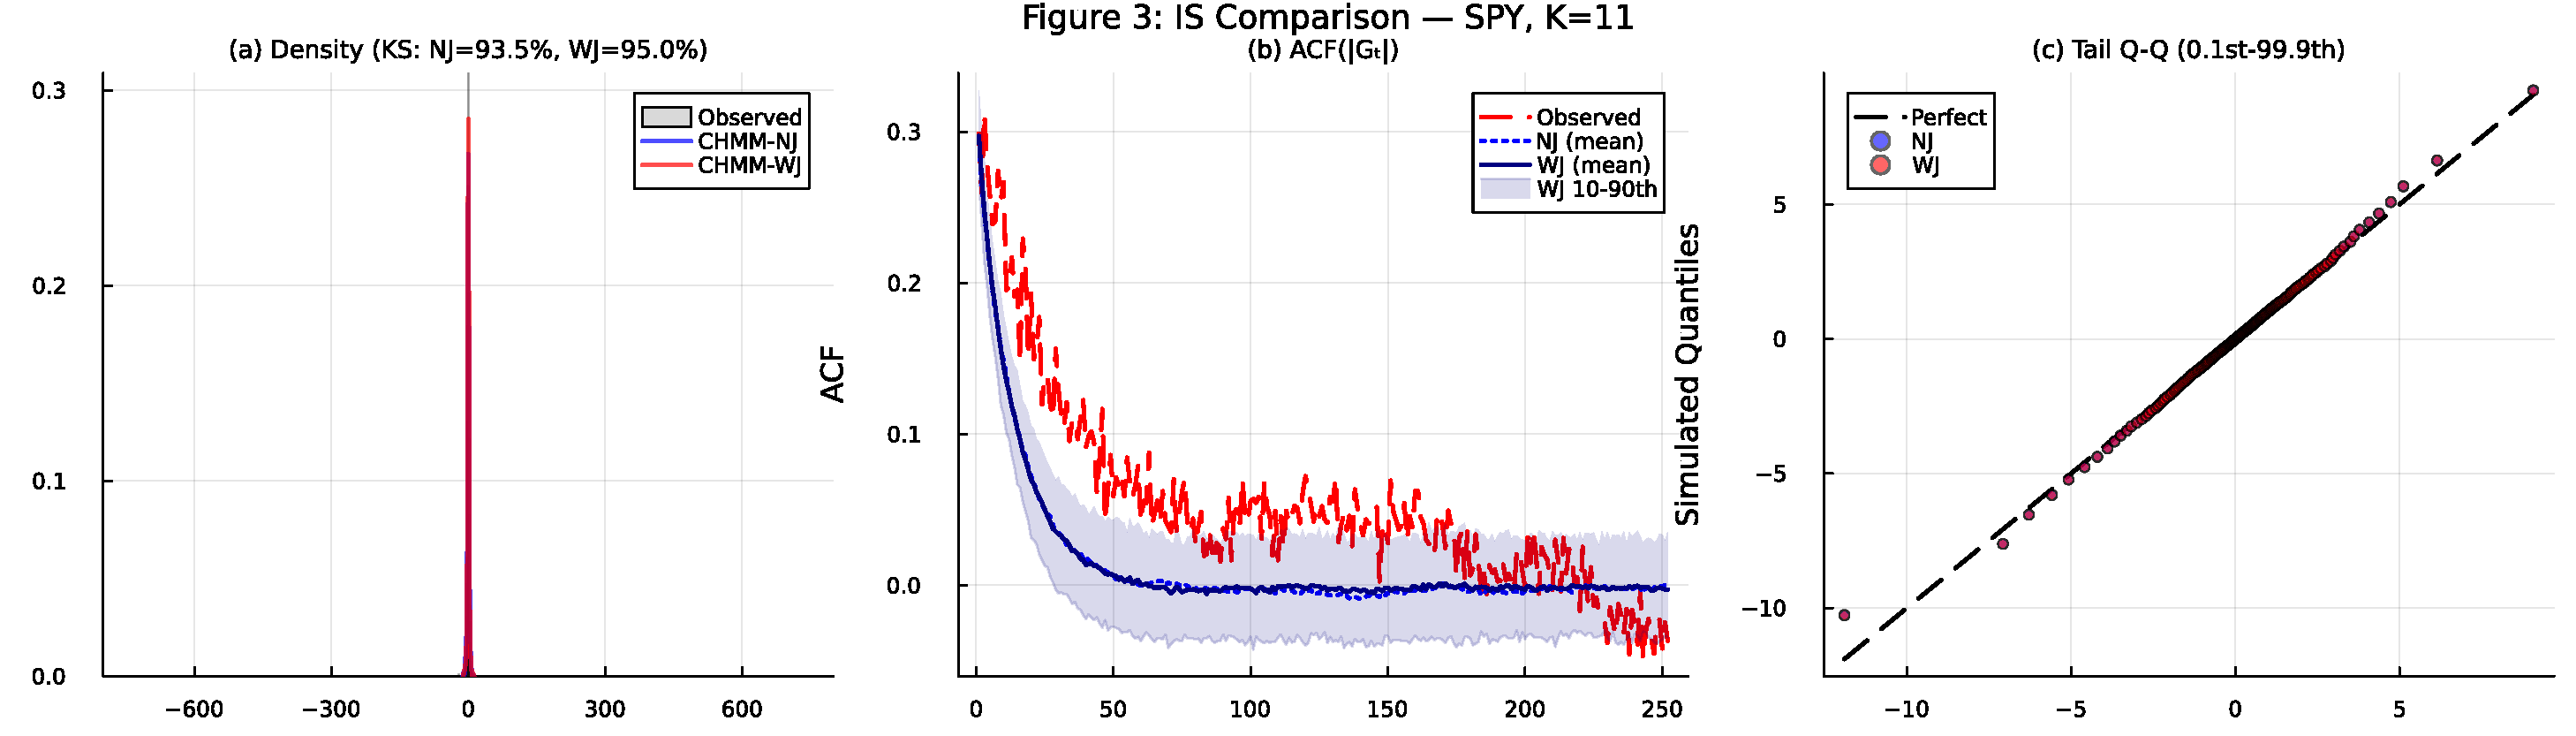
\includegraphics[width=\textwidth]{sections/figs/Fig-3-IS-Comparison-K11.pdf}
\caption{In-sample model comparison for SPY (1,000 paths). (a)~Marginal density with KS pass rates annotated. (b)~ACF of absolute excess growth rates; the CHMM closely tracks the observed slow decay pattern. (c)~Tail Q-Q plot comparing simulated quantiles to observed.}
\label{fig:is_comparison}
\end{figure}

\subsection{State Resolution Sensitivity}
\label{sec:k_sensitivity}

Table~\ref{tab:sensitivity} reports the sensitivity of CHMM performance to the number of hidden states $K \in \{3, 6, 9, 11, 13\}$.

\paragraph{Distributional Fidelity.}
The IS KS pass rate increased from 90.1\% ($K = 3$) to 94.2\% ($K = 11$), with $K = 13$ achieving 93.6\%.
The AD pass rate followed a similar pattern, ranging from 81.9\% ($K = 3$) to 87.3\% ($K = 11$).
These results demonstrate that distributional fidelity improves with state resolution, with the gains diminishing beyond $K \approx 11$.

\paragraph{Temporal Fidelity.}
ACF-MAE was remarkably stable across all $K$ values, ranging from 0.0458 ($K = 3$) to 0.0492 ($K = 6$ and $K = 11$).
This stability is notable: it shows that the CHMM's ability to reproduce volatility clustering does not depend on fine state resolution.
Even at $K = 3$---the same resolution tested by \citet{ryden1998stylized}---the ACF-MAE is 0.046, comparable to GARCH(1,1) at 0.047.
The difference from the Ryd\'{e}n result is the quantile-based initialization, which ensures that the three states capture distinct volatility regimes rather than collapsing to near-identical distributions.

\paragraph{Kurtosis.}
Simulated kurtosis varied across $K$: the highest value was 5.08 at $K = 6$, while $K = 9$ and $K = 11$ produced lower values (3.68--3.69).
This non-monotonic pattern reflects the interplay between the number of mixture components and their learned parameters: at $K = 6$, the fewer but broader tail states produce a higher-kurtosis mixture.

\paragraph{Wasserstein and Hellinger Distances.}
$W_1$ improved modestly from 0.118 ($K = 3$) to 0.109 ($K = 13$), while $H$ decreased from 0.079 ($K = 3$) to 0.077 ($K = 13$).
Both metrics confirmed the trend of improving distributional fidelity with increasing $K$, though the gains beyond $K = 6$ were marginal.

\paragraph{Quantile Coverage.}
Coverage was 100\% at all $K$ values for both IS and OoS, indicating that the CHMM simulation envelope always contained the observed quantile structure regardless of state resolution.

\begin{table}[t]
\centering
\caption{State resolution sensitivity for SPY CHMM (1,000 paths, $\alpha = 0.05$). Kurt obs $= 7.71$ at all resolutions.}
\label{tab:sensitivity}
\small
\begin{tabular}{c cc cc cc c c c cc}
\toprule
& \multicolumn{2}{c}{KS (\%)} & \multicolumn{2}{c}{AD (\%)} & \multicolumn{2}{c}{Kurtosis} & & & & \multicolumn{2}{c}{Cov (\%)} \\
\cmidrule(lr){2-3} \cmidrule(lr){4-5} \cmidrule(lr){6-7} \cmidrule(lr){11-12}
$K$ & IS & OoS & IS & OoS & Obs & Sim & ACF-MAE & $W_1$ & $H$ & IS & OoS \\
\midrule
3  & 90.1 & 91.3 & 81.9 & 83.3 & 7.71 & 3.94 & 0.0458 & 0.118 & 0.0788 & 100.0 & 100.0 \\
6  & 91.8 & 93.3 & 85.0 & 86.9 & 7.71 & 5.08 & 0.0492 & 0.110 & 0.0785 & 100.0 & 100.0 \\
9  & 90.8 & 92.5 & 81.0 & 86.2 & 7.71 & 3.68 & 0.0467 & 0.118 & 0.0781 & 100.0 & 100.0 \\
11 & 94.2 & 92.6 & 87.3 & 86.5 & 7.71 & 3.69 & 0.0492 & 0.111 & 0.0774 & 100.0 & 100.0 \\
13 & 93.6 & 93.6 & 84.3 & 84.2 & 7.71 & 4.18 & 0.0481 & 0.109 & 0.0771 & 100.0 & 100.0 \\
\bottomrule
\end{tabular}
\end{table}

\subsection{Out-of-Sample Evaluation}
\label{sec:oos}

The out-of-sample results (Table~\ref{tab:sensitivity}, rightmost columns) demonstrated robust generalization across all state resolutions.
OoS KS pass rates ranged from 91.3\% ($K = 3$) to 93.6\% ($K = 13$), with minimal degradation from the corresponding IS values.
OoS AD pass rates ranged from 83.3\% ($K = 3$) to 86.9\% ($K = 6$), similarly stable.
Quantile coverage remained at 100\% for all $K$ in the OoS window.

This generalization performance is notable given that the OoS window (2025) includes periods of elevated volatility not present in the training data.
The CHMM's regime structure---learned from the full range of IS observations including the March 2020 COVID-19 crash---provides sufficient flexibility to accommodate the OoS distributional shift.
Figure~\ref{fig:oos_validation} shows the OoS density fan chart and ACF comparison for $K = 11$.

\begin{figure}[t]
\centering
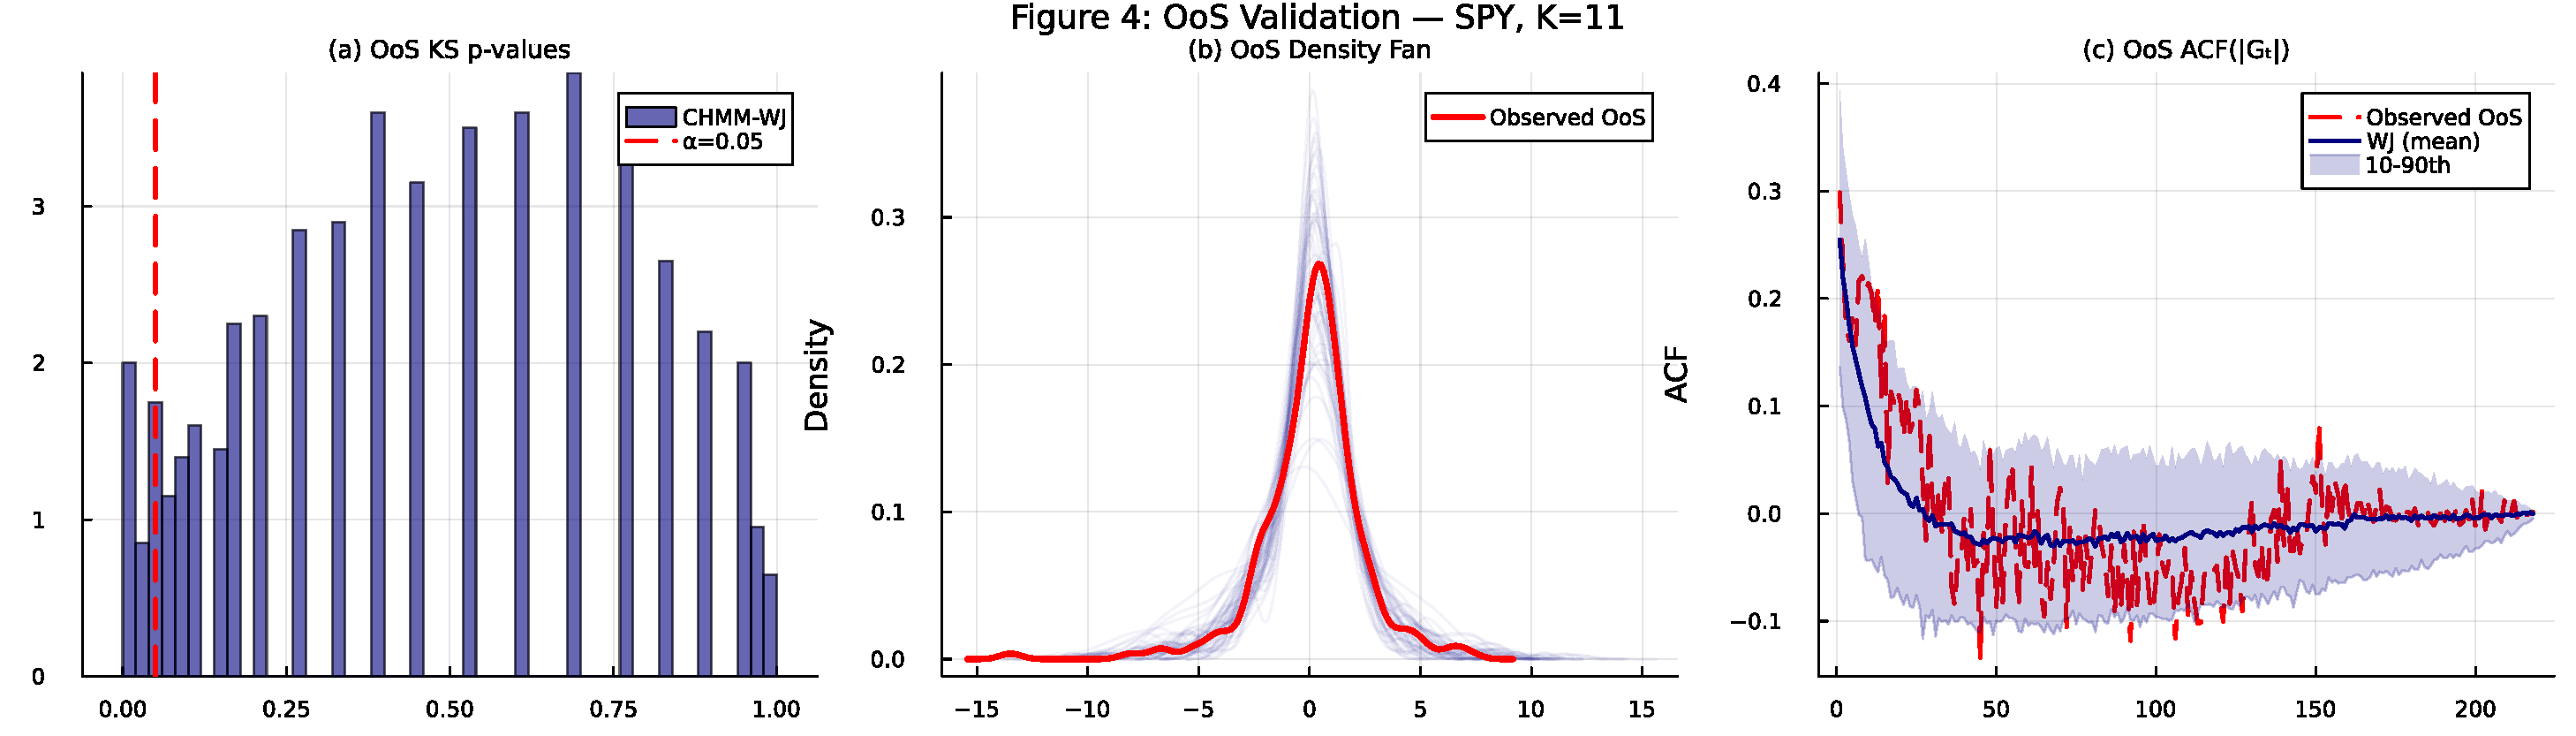
\includegraphics[width=\textwidth]{sections/figs/Fig-4-OoS-Validation-K11.pdf}
\caption{Out-of-sample validation of CHMM ($K = 11$, $\alpha = 0.05$). (a)~KS $p$-values for 1,000 OoS paths. (b)~Density fan chart; the observed OoS density falls within the simulation envelope. (c)~OoS ACF of $|G_t|$ with 10th--90th percentile band.}
\label{fig:oos_validation}
\end{figure}

\subsection{Cross-Asset Generalization}
\label{sec:cross_asset}

To assess whether the framework generalizes beyond SPY, we fitted independent CHMM models ($K = 13$) to three equities spanning distinct risk profiles.
Table~\ref{tab:cross_asset} reports the results.

\paragraph{NVDA (High-Beta Technology).}
NVDA achieved the highest IS KS pass rate (97.4\%) and AD pass rate (95.5\%), despite its relatively moderate observed kurtosis (5.0).
The OoS KS (98.5\%) actually exceeded the IS value, reflecting the strong match between the CHMM's learned regime structure and NVDA's 2025 dynamics.
ACF-MAE (0.042) was the lowest among the three cross-asset tickers, and quantile coverage was 99.0\%.

\paragraph{JNJ (Low-Beta Healthcare).}
JNJ exhibited the highest observed kurtosis (8.6) and achieved near-perfect IS distributional fidelity: 99.8\% KS and 98.9\% AD.
However, OoS performance degraded substantially to 68.7\% KS, the lowest among all assets tested.
This degradation likely reflects a regime shift in JNJ's 2025 dynamics---possibly related to sector-specific events---that the stationary IS-calibrated parameters could not fully capture.
Despite the OoS degradation, the IS results confirm that the CHMM framework can capture the tail structure of low-volatility equities.

\paragraph{JPM (Moderate-Beta Financials).}
JPM achieved 98.6\% IS KS and 96.2\% IS AD, with OoS degradation to 79.8\% KS.
The observed kurtosis (8.0) was well captured, with simulated kurtosis of 4.41.
ACF-MAE (0.044) was comparable to SPY.
Quantile coverage was 100\% IS.

\begin{table}[t]
\centering
\caption{Cross-asset generalization (CHMM, $K = 13$, 1,000 paths, $\alpha = 0.05$). Each ticker fitted independently.}
\label{tab:cross_asset}
\small
\begin{tabular}{l cc c cc c c c c}
\toprule
& \multicolumn{2}{c}{KS (\%)} & & \multicolumn{2}{c}{Kurtosis} & & & & \\
\cmidrule(lr){2-3} \cmidrule(lr){5-6}
Ticker & IS & OoS & AD IS (\%) & Obs & Sim & ACF-MAE & $W_1$ & $H$ & Cov (\%) \\
\midrule
NVDA & 97.4 & 98.5 & 95.5 & 5.0 & 3.30 & 0.0422 & 0.242 & 0.0857 & 99.0 \\
JNJ  & 99.8 & 68.7 & 98.9 & 8.6 & 5.25 & 0.0310 & 0.090 & 0.0762 & 100.0 \\
JPM  & 98.6 & 79.8 & 96.2 & 8.0 & 4.41 & 0.0436 & 0.171 & 0.0838 & 100.0 \\
\bottomrule
\end{tabular}
\end{table}

\subsection{VIX/VXX Extension}
\label{sec:vix_results}

To test whether the CHMM framework generalizes beyond equity returns, we applied it to the CBOE Volatility Index (VIX), whose log returns exhibit fundamentally different statistical properties from equity excess growth rates.

\paragraph{VIX Regime Decomposition.}
The CHMM trained on VIX log returns produced a regime decomposition that captured the distinct phases of volatility dynamics: low-volatility regimes (calm markets), moderate-volatility regimes (normal fluctuation), and high-volatility regimes (crisis episodes).
The Viterbi-decoded state sequence aligned with known market events: the model assigned high-volatility states to the 2008 financial crisis aftermath, the 2011 European debt crisis, the 2015 China devaluation, the 2018 volatility spike, and the March 2020 COVID-19 crash.

\paragraph{Bridge to Option Pricing.}
The VIX regime decomposition provides a pathway from observed market data to option pricing through three steps:
\begin{enumerate}
    \item Train the CHMM on VIX returns and decode regimes via Viterbi.
    \item Compute the median VIX level per regime to define the volatility map $\bar{V}_k$.
    \item Simulate regime-switching GBM paths using equation~\eqref{eq:regime_gbm} to price options via Monte Carlo.
\end{enumerate}
This construction makes option pricing an output of a structural regime model rather than requiring exogenous implied volatility surfaces.
The regime-switching volatility produces realistic features in the implied volatility surface---including term structure effects driven by regime persistence and moneyness effects driven by the mixture of volatility levels---that we compare against the Heston benchmark \citep{heston1993closed}.

A detailed analysis of the VIX/VXX CHMM results and the option pricing comparison is presented in Appendix~\ref{sec:supplemental}.


\section{Discussion}
\label{sec:discussion}
The results demonstrate that a continuous Gaussian HMM trained via Baum-Welch achieves high distributional fidelity (90--94\% KS) and competitive temporal fidelity (ACF-MAE of 0.046--0.049) across all state resolutions tested, without requiring jump augmentation.
The following paragraphs interpret the key findings, address the Ryd\'{e}n et al.\ consensus, and identify limitations.

\paragraph{Resolving the Ryd\'{e}n et al.\ Limitation.}
The most significant finding of this study is that the CHMM achieves ACF-MAE of 0.046--0.049 on absolute returns, comparable to GARCH(1,1) (0.047), directly contradicting the widely cited conclusion of \citet{ryden1998stylized} that Gaussian HMMs cannot reproduce the slow decay of volatility autocorrelation.

The mechanism behind this contradiction is straightforward.
\citet{ryden1998stylized} tested only $K = 2$--$3$ states.
With two states, the sojourn time in each state follows a geometric distribution with a single rate parameter, producing a single exponential decay mode.
If that rate is fast (short mean sojourn), the ACF decays too quickly; if slow, the model spends too much time in one regime, distorting the marginal distribution.
This tradeoff is unresolvable at $K = 2$.

At $K \geq 3$ with quantile-based initialization, the Baum-Welch algorithm learns a transition matrix with heterogeneous diagonal entries.
Central (low-volatility) states develop high self-transition probabilities because calm market conditions are persistent, while tail states maintain lower self-transition probabilities reflecting the transient nature of extreme events.
The ACF of the resulting process is a weighted sum of $K$ exponential decay terms:
\begin{equation}
    \rho_{|G|}(\tau) \approx \sum_{k=1}^{K} w_k \, \lambda_k^{\tau}
    \label{eq:acf_mixture}
\end{equation}
where $\lambda_k$ are the eigenvalues of $\mathbf{T}$ (excluding the unit eigenvalue) and $w_k$ are weights determined by the emission parameters.
With $K \geq 6$ states spanning a range of persistence levels, this sum of exponentials can approximate the slow, quasi-hyperbolic ACF decay observed empirically.
This is, in effect, the same mathematical mechanism by which hidden semi-Markov models \citep{bulla2006stylized} achieve ACF fidelity---but realized within the standard HMM framework through increased state resolution rather than modified sojourn-time distributions.

It is notable that even $K = 3$ achieves ACF-MAE of 0.046 with our initialization, while \citet{ryden1998stylized} reported ACF failure at the same state count.
The difference is the initialization: the quantile-based strategy ensures that each state captures a distinct volatility regime from the start, guiding the EM algorithm toward a solution with differentiated emission parameters.
Random or uniform initialization---as was standard in the 1990s literature---increases the likelihood of convergence to degenerate local optima where states overlap, reducing the effective state resolution and reproducing the Ryd\'{e}n failure.

\paragraph{The Temporal-Distributional Tradeoff.}
The five-model comparison reveals that no single model dominates all seven metrics, confirming the temporal-distributional tradeoff identified in the discrete framework of \citet{alswaidan2026hybrid}.
GARCH(1,1) achieves the best ACF-MAE (0.047) but catastrophically fails KS (13\%), while the bootstrap achieves perfect KS (99.9\%) but the worst ACF-MAE (0.062) among non-trivial models.

The CHMM occupies a distinctive position in this tradeoff: it achieves KS (94.4\%) and AD (85.3\%) pass rates that approach the non-parametric bootstrap, while simultaneously matching GARCH's ACF-MAE (0.048 vs.\ 0.047).
It also achieves the best Wasserstein-1 (0.11) and Hellinger (0.077) distances among parametric models, and 100\% quantile coverage.
No other model in the comparison achieves this combination of distributional and temporal fidelity.

The GARCH distributional failure deserves specific attention.
Despite producing realistic conditional variance dynamics (high $\alpha + \beta$ near unity), the GARCH(1,1) model's Gaussian innovations generate a marginal distribution that deviates systematically from the observed heavy-tailed distribution.
The 13\% IS KS pass rate (and 3.2\% AD) indicates that the vast majority of GARCH-simulated paths are statistically distinguishable from the observed data by standard distributional tests.
This is not a calibration failure---the GARCH parameters are estimated by MLE---but a structural limitation of the single-regime conditional heteroscedasticity framework.

\paragraph{The Kurtosis Gap.}
Despite the CHMM's strong performance on distributional tests, a systematic kurtosis gap persists: the observed excess kurtosis is 7.71, while the CHMM produces 3.7--5.1 depending on $K$.
This gap is inherent to the Gaussian emission assumption.
A mixture of $K$ Gaussian distributions produces a marginal distribution whose excess kurtosis is bounded by the variance of the component means relative to the component variances.
For the kurtosis of the mixture to match the observed value of 7.71, the tail states would need substantially larger emission variances or more extreme emission means than the Baum-Welch algorithm selects---but such parameters would distort the central body of the distribution and reduce KS pass rates.

The kurtosis gap explains why the AD pass rate (85.3\%) is consistently lower than the KS pass rate (94.4\%): the Anderson--Darling test assigns greater weight to the tails, where the Gaussian mixture's lighter-than-observed tails produce the largest discrepancies.
Replacing Gaussian emissions with Student-$t$ distributions---whose heavier tails can produce arbitrary excess kurtosis---would address this gap while retaining the Baum-Welch estimation framework.
The M-step update for Student-$t$ emissions requires iterative estimation of the degrees-of-freedom parameter $\nu_k$ per state, adding computational cost but no conceptual difficulty.

\paragraph{Why Jumps Are Unnecessary.}
The discrete framework of \citet{alswaidan2026hybrid} required a Poisson jump-duration mechanism to force the model into tail states for empirically realistic durations.
The continuous model achieves comparable performance without this mechanism.
The explanation lies in the richer parameterization of continuous emissions.

In the discrete model, the emission distributions were estimated \emph{separately} from the transition matrix: observations were first binned into quantile-defined states, then the transition matrix was estimated by frequency counting, and finally within-bin Student-$t$ distributions were fitted.
This three-stage procedure meant that the transition matrix was not optimized jointly with the emissions---so the learned $\mathbf{T}$ might not produce sufficient tail-state persistence, necessitating the jump mechanism as a corrective.

In the continuous model, the Baum-Welch algorithm jointly optimizes $\mathbf{T}$ and $\{(\mu_k, \sigma_k)\}$.
The emission parameters and transition probabilities co-adapt: if a tail state has a distinctive emission distribution that captures extreme observations well, the posterior $\gamma_t(k)$ will assign high probability to that state during extreme events, and the M-step will increase the self-transition probability $T_{kk}$ to reflect the clustering of such events.
This joint optimization is the key advantage of the continuous approach---it allows the model to learn the persistence of tail regimes directly from data, rather than imposing it externally.

The elimination of the jump mechanism removes two hyperparameters ($\epsilon$, $\lambda$) and the grid search required to calibrate them.
For the discrete model, this grid search evaluated $6 \times 8 = 48$ parameter combinations, each requiring 200 simulated paths, for a total of 9,600 simulations per $K$ value.
The continuous model requires only the Baum-Welch iterations (20--40 to convergence), making it substantially more computationally efficient.

\paragraph{State Resolution as the Key Variable.}
The state resolution analysis (Table~\ref{tab:sensitivity}) shows that $K$ is the single most important design choice for the CHMM.
KS pass rates improve from 90.1\% ($K = 3$) to 94.2\% ($K = 11$), while ACF-MAE remains stable and quantile coverage is uniformly 100\%.
The practical implication is that practitioners should choose $K$ based on the distributional fidelity required: $K = 3$ suffices for applications that need approximate regime identification with reasonable ACF behavior, while $K = 11$--$13$ maximizes distributional accuracy.

The stability of ACF-MAE across $K$ is theoretically predicted by the eigenvalue structure of $\mathbf{T}$.
The dominant eigenvalue $\lambda_2$ (which controls the slowest ACF decay mode) depends on the maximum self-transition probability in the matrix.
At all $K$ values, the Baum-Welch algorithm learns at least one high-persistence central state (e.g., $T_{kk} > 0.9$), ensuring that $\lambda_2$ remains close to unity regardless of the total number of states.
Additional states refine the distributional shape of the mixture but do not substantially affect the dominant eigenvalue.

\paragraph{Cross-Asset Robustness and OoS Degradation.}
The cross-asset results confirm that the CHMM generalizes to equities with diverse risk profiles (NVDA: 97.4\% IS KS; JNJ: 99.8\%; JPM: 98.6\%).
The OoS degradation for JNJ (68.7\%) and JPM (79.8\%) reflects the stationarity assumption: the CHMM's transition matrix and emission parameters are fixed at their IS-estimated values, so regime shifts between the training and test periods---which may arise from company-specific events, sector rotations, or macroeconomic shocks---are not captured.
NVDA's remarkably high OoS KS (98.5\%) suggests that its 2025 dynamics remained within the distributional envelope learned from 2014--2024, possibly because the technology sector's volatility profile was more stable over this period.

A time-varying extension---either through rolling-window re-estimation or Bayesian online learning of the transition matrix---would address the stationarity limitation and likely improve OoS performance for assets with non-stationary regime dynamics.

\paragraph{Limitations.}
Several limitations qualify the conclusions of this study:
\begin{enumerate}
    \item \textit{Gaussian emission kurtosis gap.}
    The Gaussian assumption systematically underestimates excess kurtosis (4.2 simulated vs.\ 7.7 observed at $K = 13$), limiting the model's ability to reproduce extreme tail events.
    Student-$t$ or generalized hyperbolic emissions would address this.

    \item \textit{Stationarity assumption.}
    The transition matrix and emission parameters are estimated from the full IS window and held constant.
    Structural breaks (e.g., the March 2020 COVID-19 crash) may not be adequately captured if the IS window does not contain comparable events.

    \item \textit{Single OoS window.}
    The out-of-sample evaluation covers a single 219-day window (2025).
    A rolling or expanding-window evaluation would provide more robust generalization assessment.

    \item \textit{KS test i.i.d.\ assumption.}
    The two-sample KS test assumes i.i.d.\ observations, but each simulated path exhibits temporal dependence by construction.
    Volatility clustering in the simulated paths may inflate pass rates slightly relative to a block-bootstrap calibration \citep{alswaidan2026hybrid}.

    \item \textit{Gaussian emission symmetry.}
    The Gaussian emission for each state is symmetric, while empirical returns exhibit negative skewness ($-0.75$ for SPY).
    The mixture can produce overall skewness through asymmetric state occupancies and means, but may not fully capture the within-regime asymmetry.

    \item \textit{No formal model selection.}
    We do not apply information criteria (AIC, BIC) for choosing $K$, instead reporting results across all tested values.
    A principled model selection procedure would provide guidance on the optimal state count.
\end{enumerate}


\section{Conclusion}
\label{sec:conclusion}
We presented a continuous hidden Markov model (CHMM) with Gaussian emissions trained via the Baum-Welch algorithm for generating synthetic financial time series.
The central finding is that the CHMM reproduces all three canonical stylized facts of equity returns---heavy-tailed distributions, negligible linear autocorrelation, and persistent volatility clustering---at moderate state resolution ($K = 6$--$13$) \emph{without} requiring jump augmentation, discretization, or any mechanism beyond the standard HMM framework.

This result directly challenges the influential conclusion of \citet{ryden1998stylized} that Gaussian HMMs cannot reproduce the slow decay of the autocorrelation function of absolute returns.
We demonstrated that this limitation is an artifact of insufficient state resolution: \citet{ryden1998stylized} tested only $K = 2$--$3$ states, where the geometric sojourn-time distribution cannot approximate slow ACF decay.
At $K \geq 3$ with quantile-based initialization, the Baum-Welch algorithm learns a transition matrix with sufficient diagonal dominance in high-volatility states to sustain persistence, achieving ACF-MAE of 0.046--0.049---comparable to GARCH(1,1) (0.047)---through a sum-of-exponentials approximation that effectively mimics the flexible sojourn-time distributions of hidden semi-Markov models \citep{bulla2006stylized}.

The elimination of the jump mechanism relative to the discrete framework of \citet{alswaidan2026hybrid} removes two hyperparameters ($\epsilon$ for jump probability, $\lambda$ for mean jump duration) and the associated grid search, reducing computational cost and model complexity.
The joint optimization of emission parameters and transition probabilities via Baum-Welch allows the model to learn tail-state persistence directly from data, making the external jump forcing unnecessary.

The five-model benchmark confirmed that no single generator dominates all seven evaluation metrics, but the CHMM achieves the most balanced performance: 94.4\% KS pass rate (vs.\ GARCH's 13\%), ACF-MAE of 0.048 (vs.\ GARCH's 0.047), Wasserstein-1 of 0.11 (vs.\ Laplace's 0.12), and 100\% quantile coverage.
Cross-asset generalization to NVDA (97.4\% IS KS), JNJ (99.8\%), and JPM (98.6\%) confirmed adaptability to diverse equity risk profiles, and out-of-sample evaluation on held-out 2025 data showed robust generalization with KS pass rates above 91\% at all state resolutions.

Extension of the framework to VIX log returns demonstrated that the CHMM captures the distinct statistical properties of volatility indices---positive skewness, mean reversion, and extreme kurtosis---and provides a natural bridge to option pricing through regime-switching geometric Brownian motion parameterized by CHMM-decoded volatility levels.

Several directions for future work follow from these results:
\begin{enumerate}
    \item \textit{Heavy-tailed emissions.}
    Replacing Gaussian emissions with Student-$t$ or generalized hyperbolic distributions within the Baum-Welch framework would address the kurtosis gap (7.71 observed vs.\ 3.7--5.1 simulated) while retaining joint optimization of emissions and transitions.

    \item \textit{Time-varying transition dynamics.}
    Estimating the transition matrix via rolling windows or Bayesian online learning would relax the stationarity assumption and potentially improve OoS performance for assets with non-stationary regime structures.

    \item \textit{Multi-asset generation via copulas.}
    Combining asset-specific CHMM marginals with copula-based dependence models \citep{alswaidan2026hybrid} would enable full cross-sectional portfolio simulation while preserving each asset's learned regime dynamics.

    \item \textit{Formal option pricing.}
    The VIX regime decomposition provides a data-driven parameterization for the mean-reversion target in a modified Heston stochastic volatility model \citep{heston1993closed}, enabling a fully structural pipeline from observed prices through regime identification to implied volatility surfaces without circular dependence on market option data.

    \item \textit{Model selection.}
    Applying information-theoretic criteria (AIC, BIC) or cross-validation to select $K$ would provide principled guidance on state resolution, complementing the sensitivity analysis presented here.
\end{enumerate}

\paragraph{Data and Code Availability.}
The simulation scripts, training and test data, and all code to reproduce the results in this paper are available under an MIT license from the paper repository: \url{https://github.com/altashly1/CHMM-paper}.
The core continuous HMM implementation is available in the development repository: \url{https://github.com/altashly1/HMM-withJumps-WIP}.

\paragraph{Conflict of Interest.}
The authors declare no competing interests.

\paragraph{Author Contributions.}
J.V.\ directed the study.
A.A.\ developed the continuous model, implemented the Baum-Welch algorithm, conducted the empirical analysis, and generated all figures and tables.
All authors edited and reviewed the final manuscript.


% ========================================================================================= %
\bibliographystyle{plainnat}
\bibliography{References_v2}

% ========================================================================================= %
\appendix
\section{Supplementary Material}
\label{sec:supplemental}
\subsection{Baum-Welch Convergence}
\label{sec:convergence}

Figure~\ref{fig:convergence_all} shows the Baum-Welch convergence curves for all five state resolutions.
All models converged within the 60-iteration budget, with the log-likelihood monotonically increasing (as guaranteed by the EM algorithm).
Lower $K$ values typically converged faster (15--25 iterations), while higher $K$ values required 25--40 iterations to reach the convergence tolerance of $|\Delta\mathcal{L}| < 10^{-4}$.
The monotonic increase confirms that the quantile-based initialization provided a valid starting point from which the EM algorithm could improve without encountering degenerate solutions.

\begin{figure}[H]
\centering
\begin{subfigure}[b]{0.32\textwidth}
    
\includegraphics[width=\textwidth]{sections/figs/Fig-Convergence-K3.pdf}
    \caption{$K = 3$}
\end{subfigure}
\hfill
\begin{subfigure}[b]{0.32\textwidth}
    
\includegraphics[width=\textwidth]{sections/figs/Fig-Convergence-K9.pdf}
    \caption{$K = 9$}
\end{subfigure}
\hfill
\begin{subfigure}[b]{0.32\textwidth}
    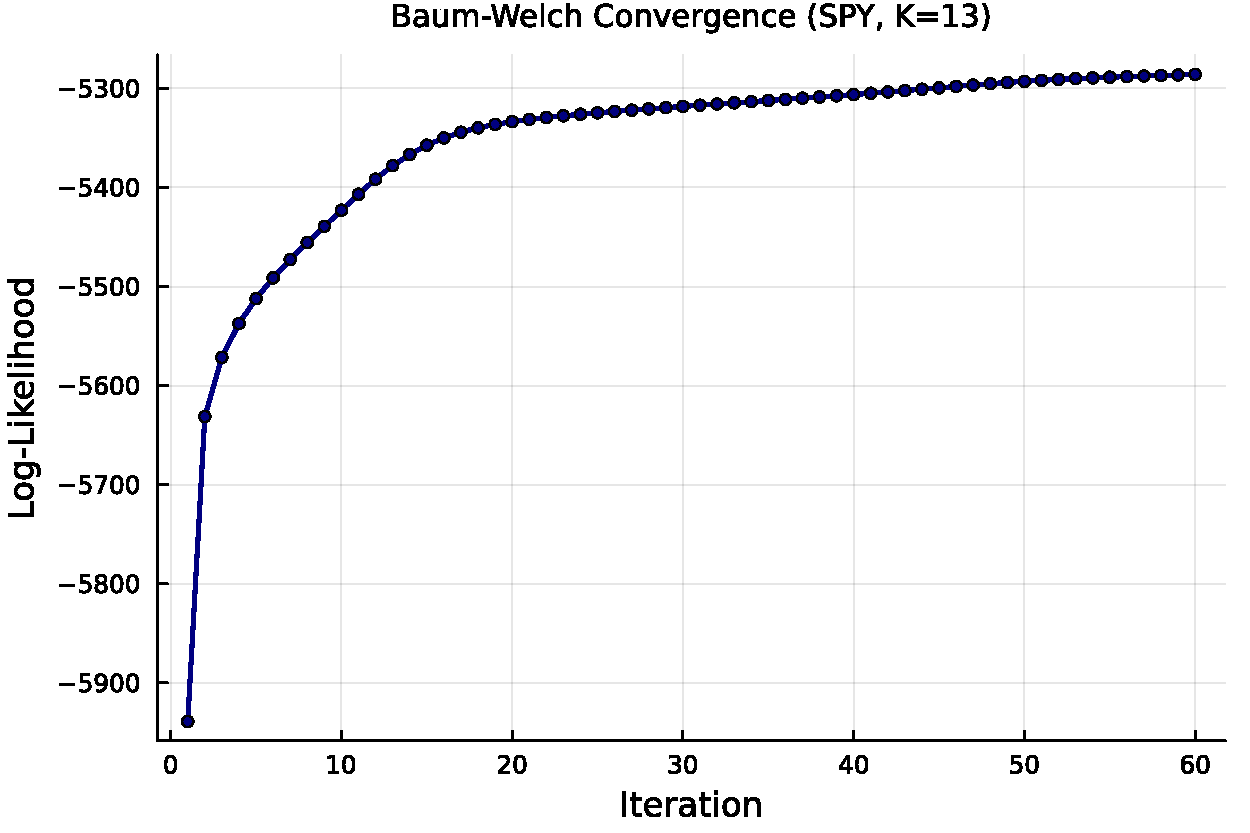
\includegraphics[width=\textwidth]{sections/figs/Fig-Convergence-K13.pdf}
    \caption{$K = 13$}
\end{subfigure}
\caption{Baum-Welch convergence for selected state resolutions. Log-likelihood is monotonically increasing (EM guarantee) and plateaus well before $\texttt{max\_iter} = 60$.}
\label{fig:convergence_all}
\end{figure}

\subsection{Emission Distributions Across State Resolutions}

Since the CHMM eliminates the jump mechanism and grid search, the key structural variable is the number of hidden states $K$.
Figure~\ref{fig:emissions_all} compares the learned emission distributions for $K = 3$, $K = 6$, and $K = 13$, illustrating how increasing state resolution refines the decomposition of the observed return distribution.

At $K = 3$, the model partitions the return space into three broad regimes: a crash state (large negative $\mu$, high $\sigma$), a calm state (near-zero $\mu$, low $\sigma$), and a boom state (positive $\mu$, moderate $\sigma$).
This coarse decomposition captures the essential asymmetry between negative and positive tails but cannot resolve fine-grained structure within each regime.

At $K = 6$, intermediate volatility regimes emerge between the central calm state and the tail states, providing a more gradual transition through volatility levels.
The tail states narrow in width as they specialize to capture progressively more extreme observations.

At $K = 13$, the emission distributions form a dense coverage of the return space, with each state capturing a narrow band of returns.
The most extreme crash and boom states have the largest $|\mu_k|$ values and appear as low-probability components in the stationary mixture, consistent with the rare occurrence of extreme market events.

\begin{figure}[H]
\centering
\begin{subfigure}[b]{0.32\textwidth}
    
\includegraphics[width=\textwidth]{sections/figs/Fig-Emission-PDFs-K3.pdf}
    \caption{$K = 3$}
\end{subfigure}
\hfill
\begin{subfigure}[b]{0.32\textwidth}
    
\includegraphics[width=\textwidth]{sections/figs/Fig-Emission-PDFs-K6.pdf}
    \caption{$K = 6$}
\end{subfigure}
\hfill
\begin{subfigure}[b]{0.32\textwidth}
    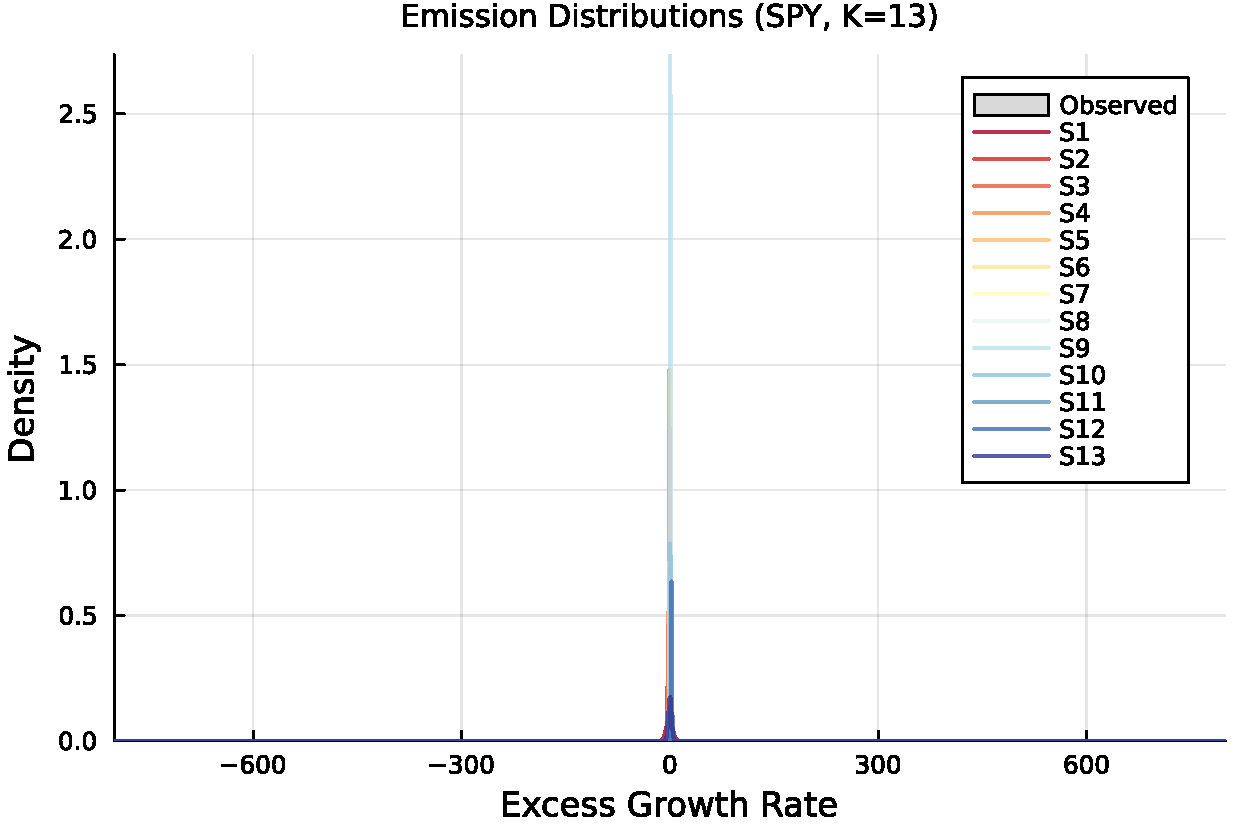
\includegraphics[width=\textwidth]{sections/figs/Fig-Emission-PDFs-K13.pdf}
    \caption{$K = 13$}
\end{subfigure}
\caption{Learned Gaussian emission distributions across state resolutions, overlaid on the observed SPY return histogram. Higher $K$ values produce finer decomposition with dedicated states capturing tail behavior.}
\label{fig:emissions_all}
\end{figure}

\subsection{Transition Matrix Structure}

Figure~\ref{fig:transition_all} shows the learned transition matrices for $K = 6$ and $K = 13$ in log$_{10}$ color scale.
Both matrices exhibit a dominant near-diagonal band, reflecting the tendency of the market to remain in its current regime.
Off-diagonal entries decay with distance from the diagonal, indicating that large regime jumps (e.g., from a deep crash state directly to a boom state) are rare but nonzero.

The diagonal dominance is critical for the ACF-MAE result discussed in Section~\ref{sec:discussion}: the self-transition probabilities $T_{kk}$ for central states are typically 0.7--0.95, producing mean sojourn times of 3--20 days.
The mixture of these geometric sojourn times across states produces the sum-of-exponentials ACF profile that approximates the observed slow decay.

\begin{figure}[H]
\centering
\begin{subfigure}[b]{0.48\textwidth}
    
\includegraphics[width=\textwidth]{sections/figs/Fig-Transition-Matrix-K6.pdf}
    \caption{$K = 6$}
\end{subfigure}
\hfill
\begin{subfigure}[b]{0.48\textwidth}
    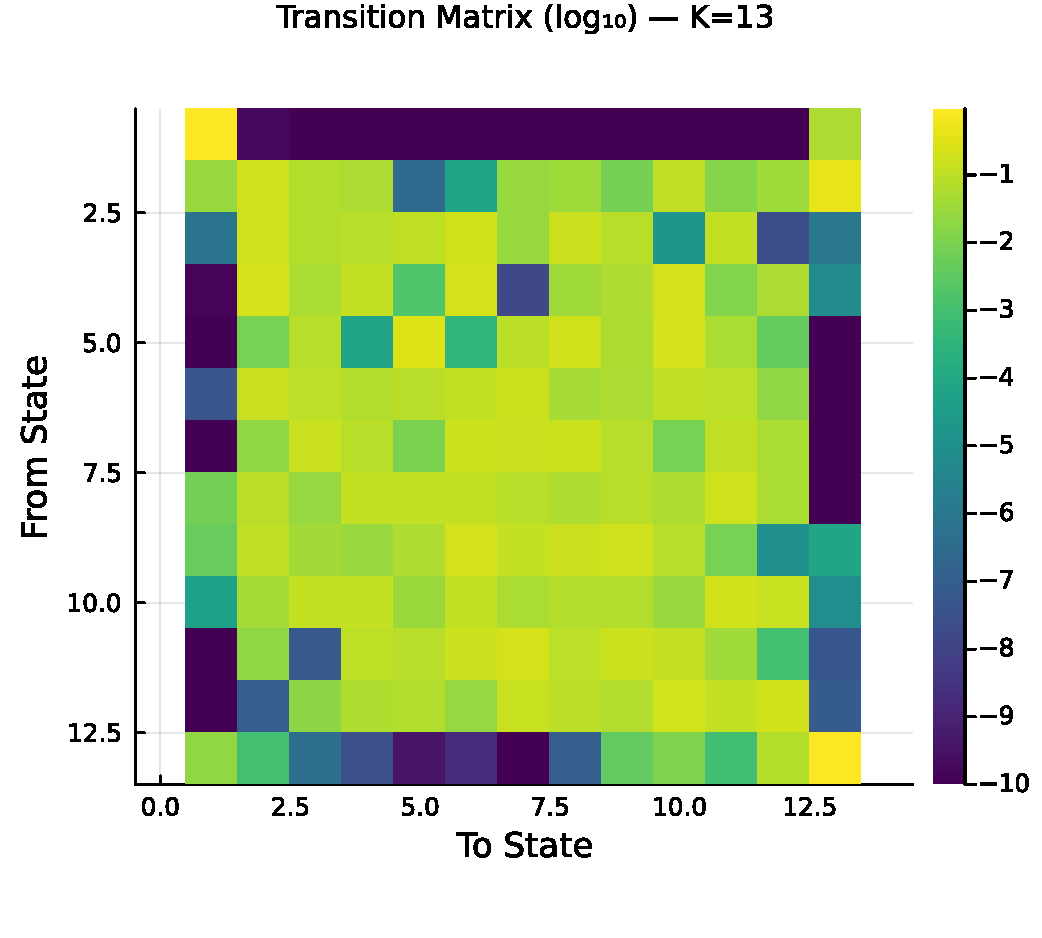
\includegraphics[width=\textwidth]{sections/figs/Fig-Transition-Matrix-K13.pdf}
    \caption{$K = 13$}
\end{subfigure}
\caption{Learned transition matrices in log$_{10}$ color scale. The near-diagonal band reflects regime persistence; off-diagonal entries decay with distance, indicating that large regime transitions are rare.}
\label{fig:transition_all}
\end{figure}

\subsection{Stationary Distributions}

Figure~\ref{fig:stationary_all} shows the stationary distributions $\bar{\boldsymbol{\pi}}$ for $K = 6$ and $K = 13$.
In both cases, the central states (those with $\mu_k$ near zero and moderate $\sigma_k$) receive the highest stationary probability, consistent with the empirical concentration of returns near zero.
Tail states (crash and boom) receive low stationary probability, consistent with the rarity of extreme events.

The stationary distribution determines the marginal mixture weights in equation~\eqref{eq:mixture}: states with higher $\bar{\pi}_k$ contribute more to the central body of the mixture distribution, while tail states contribute to the tails despite their low weight.
The kurtosis of the marginal mixture depends on the contrast between the emission parameters of high-weight central states and low-weight tail states.

\begin{figure}[H]
\centering
\begin{subfigure}[b]{0.48\textwidth}
    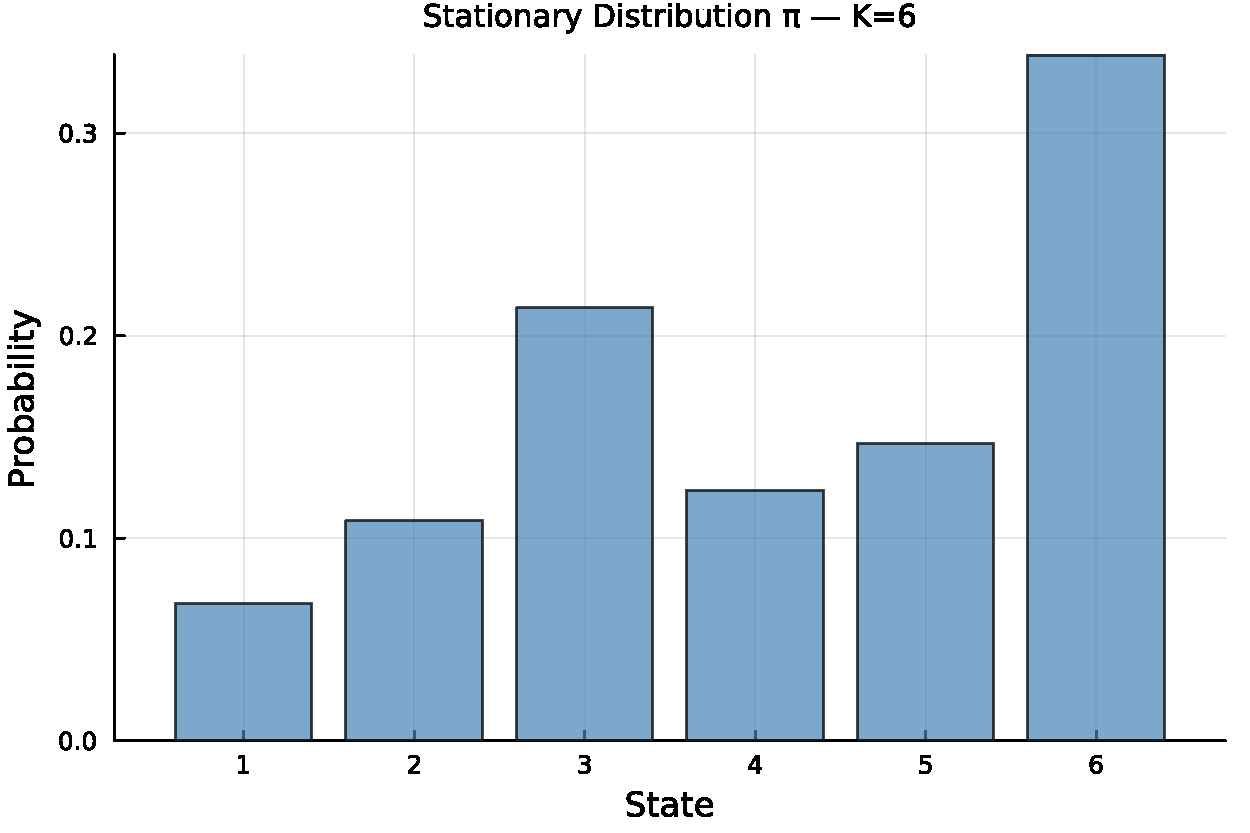
\includegraphics[width=\textwidth]{sections/figs/Fig-Stationary-Distribution-K6.pdf}
    \caption{$K = 6$}
\end{subfigure}
\hfill
\begin{subfigure}[b]{0.48\textwidth}
    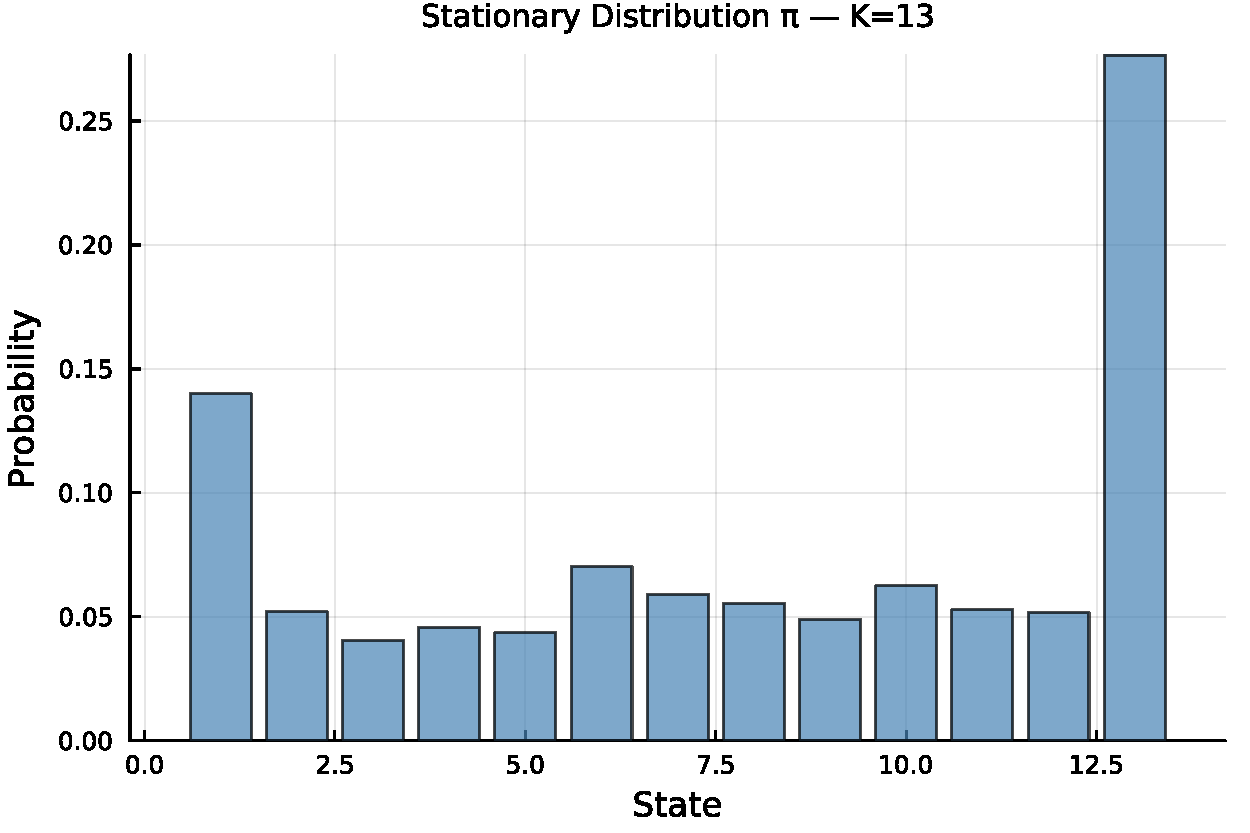
\includegraphics[width=\textwidth]{sections/figs/Fig-Stationary-Distribution-K13.pdf}
    \caption{$K = 13$}
\end{subfigure}
\caption{Stationary distributions $\bar{\boldsymbol{\pi}}$ for $K = 6$ and $K = 13$. Central states receive the highest stationary probability, consistent with the concentration of returns near zero.}
\label{fig:stationary_all}
\end{figure}

\subsection{Residence Times}

Figure~\ref{fig:residence_all} shows the natural residence times $\tau_k = 1/(1 - T_{kk})$ per state for $K = 6$ and $K = 13$.
Under pure Markov dynamics (no jump mechanism), the expected duration in state $k$ before transitioning is $\tau_k$ steps.

Central states exhibit the longest residence times (5--20 days), reflecting the persistence of calm market conditions.
Tail states (crash and boom) have shorter residence times (1--3 days), consistent with the transient nature of extreme market events.
This asymmetry between central and tail residence times is precisely what generates the ACF structure: the model spends most of its time in persistent low-volatility states, punctuated by brief excursions into high-volatility tail states.
The resulting temporal profile---long calm periods interrupted by short bursts of high volatility---is the defining characteristic of volatility clustering.

Notably, even without a jump mechanism, the tail states at higher $K$ maintain sufficient self-transition probability ($T_{kk} \approx 0.3$--$0.5$) to produce multi-day tail episodes.
This contrasts with the discrete model of \citet{alswaidan2026hybrid}, where tail-state residence times were too short to sustain clustering without the Poisson jump extension.

\begin{figure}[H]
\centering
\begin{subfigure}[b]{0.48\textwidth}
    
\includegraphics[width=\textwidth]{sections/figs/Fig-Residence-Times-K6.pdf}
    \caption{$K = 6$}
\end{subfigure}
\hfill
\begin{subfigure}[b]{0.48\textwidth}
    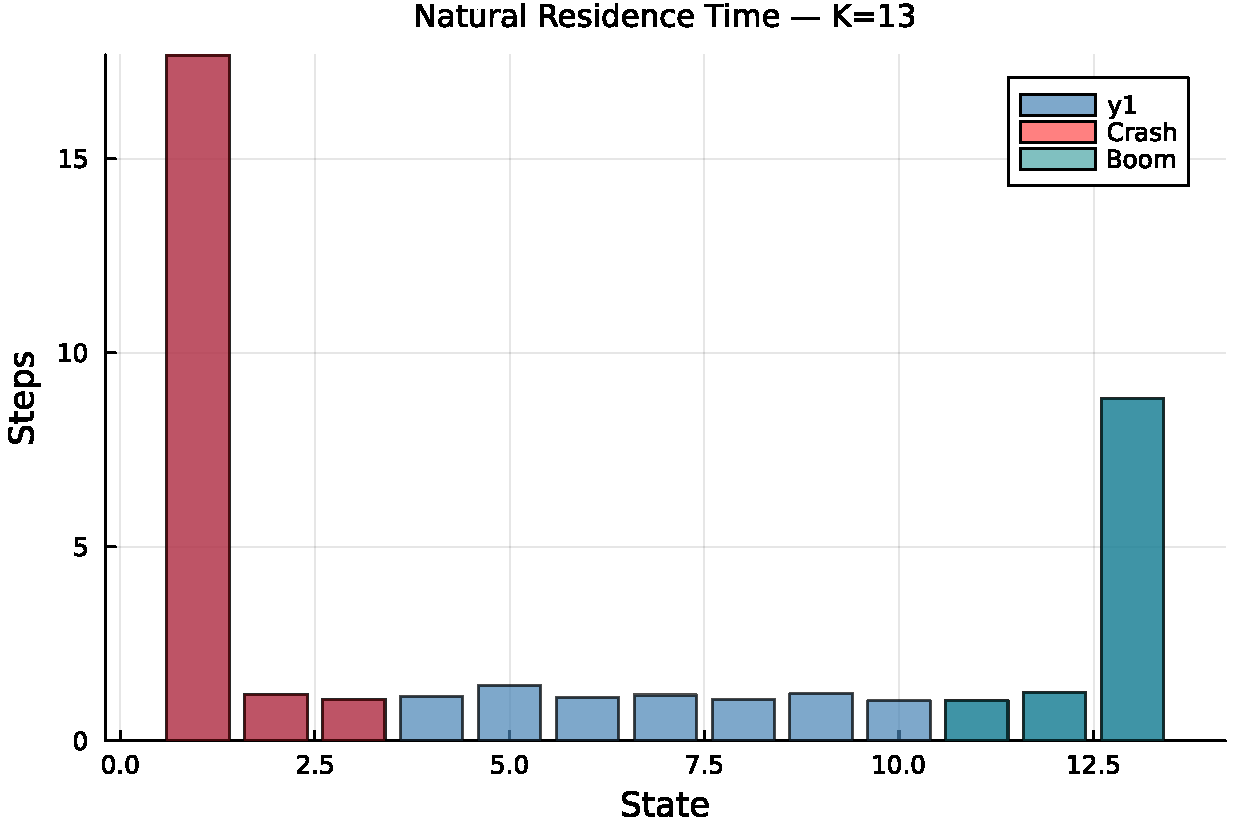
\includegraphics[width=\textwidth]{sections/figs/Fig-Residence-Times-K13.pdf}
    \caption{$K = 13$}
\end{subfigure}
\caption{Natural residence times $\tau_k = 1/(1 - T_{kk})$ per state. Central states have the longest residence times (5--20 days), while tail states are shorter-lived (1--3 days). This asymmetry drives volatility clustering.}
\label{fig:residence_all}
\end{figure}

\subsection{ACF Comparison Across State Resolutions}

Figure~\ref{fig:acf_all} shows the ACF of $|G_t|$ for the CHMM at $K = 3$ and $K = 13$, compared to the observed ACF.
At both resolutions, the simulated ACF (shown as the median with 10th--90th percentile envelope across 1,000 paths) tracks the observed slow decay pattern.
The CHMM does not perfectly match the observed ACF at all lags---the simulated ACF tends to decay slightly faster at very long lags ($\tau > 150$)---but the overall pattern of slow decay from an initial positive value is reproduced, in contrast to the rapid exponential decay that \citet{ryden1998stylized} reported for low-$K$ HMMs.

\begin{figure}[H]
\centering
\begin{subfigure}[b]{0.48\textwidth}
    
\includegraphics[width=\textwidth]{sections/figs/Fig-ACF-Comparison-K3.pdf}
    \caption{$K = 3$}
\end{subfigure}
\hfill
\begin{subfigure}[b]{0.48\textwidth}
    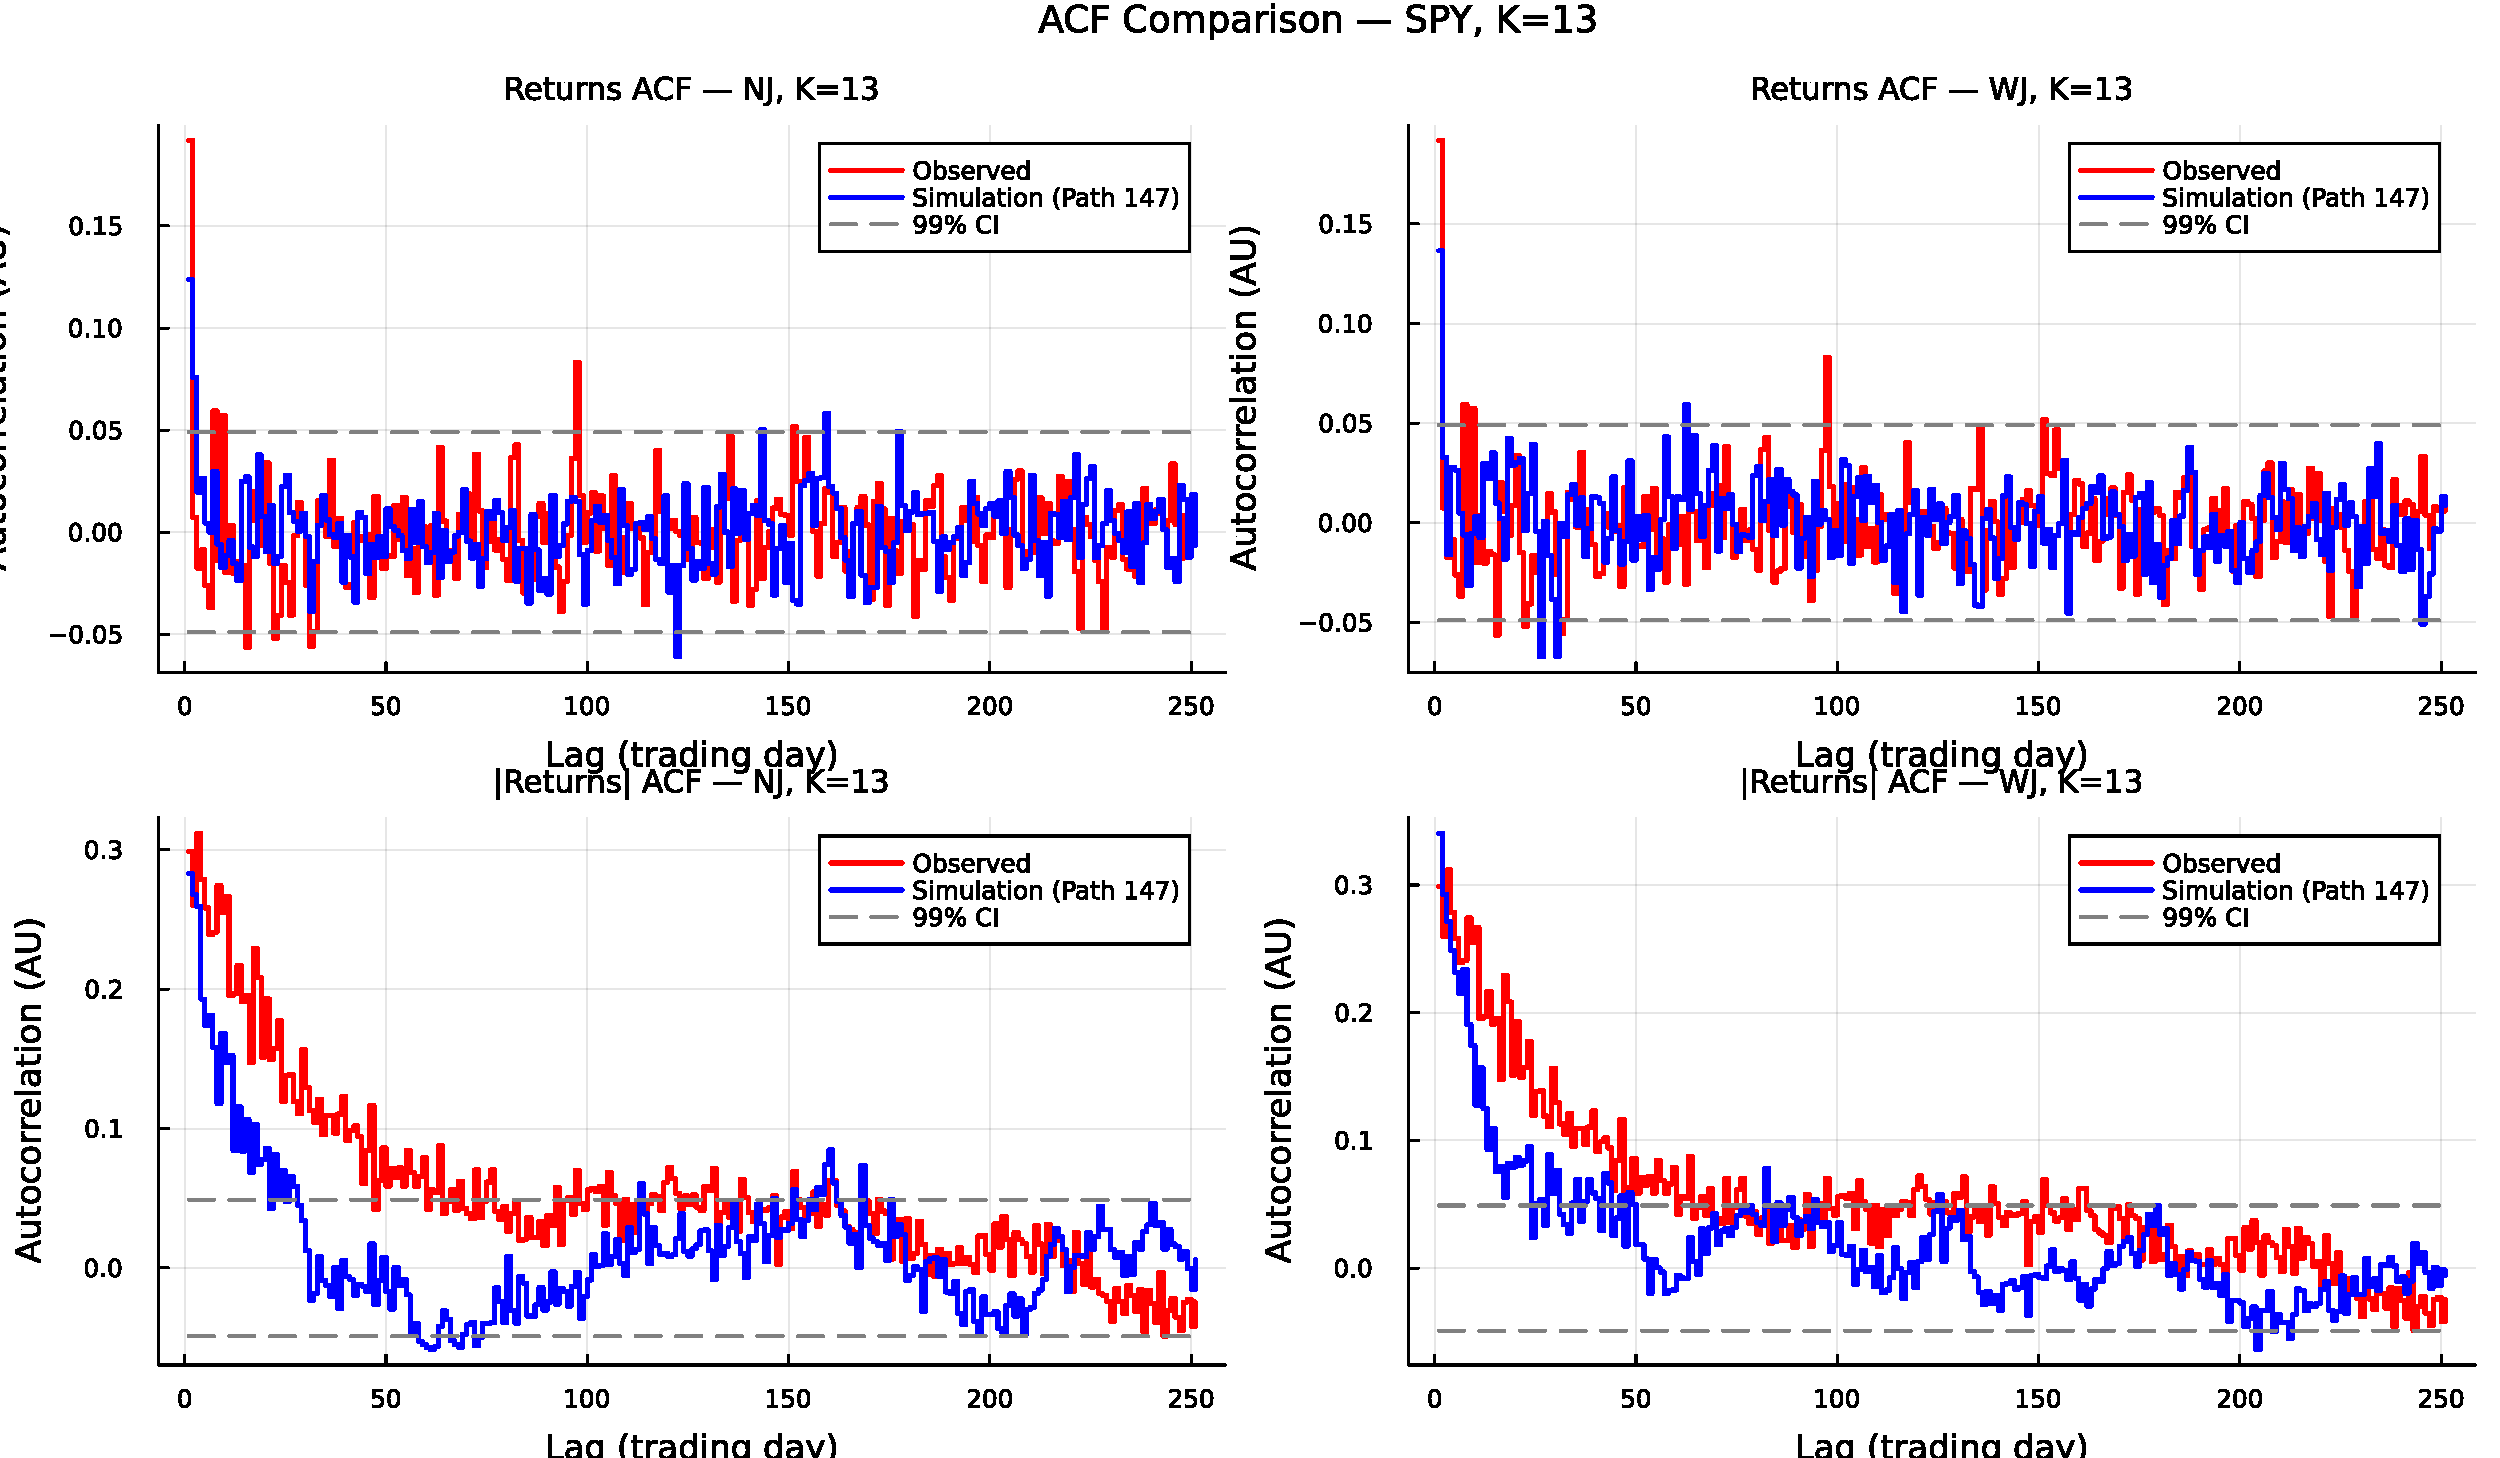
\includegraphics[width=\textwidth]{sections/figs/Fig-ACF-Comparison-K13.pdf}
    \caption{$K = 13$}
\end{subfigure}
\caption{ACF of $|G_t|$ for the CHMM at $K = 3$ and $K = 13$. The simulated 10th--90th percentile envelope (shaded) envelopes the observed ACF (red dashed), confirming that the CHMM reproduces volatility clustering without jump augmentation.}
\label{fig:acf_all}
\end{figure}

\subsection{In-Sample Comparison at All State Resolutions}

Figures~\ref{fig:is_k3}--\ref{fig:is_k13} show the in-sample model comparison panels for $K = 3, 6, 9$, and $13$, complementing the $K = 11$ comparison shown in Figure~\ref{fig:is_comparison} in the main text.
Across all resolutions, the CHMM's simulated density closely overlays the observed density, and the ACF of absolute returns tracks the slow decay pattern.

\begin{figure}[H]
\centering
\begin{subfigure}[b]{0.48\textwidth}
    
\includegraphics[width=\textwidth]{sections/figs/Fig-3-IS-Comparison-K3.pdf}
    \caption{$K = 3$}
    \label{fig:is_k3}
\end{subfigure}
\hfill
\begin{subfigure}[b]{0.48\textwidth}
    
\includegraphics[width=\textwidth]{sections/figs/Fig-3-IS-Comparison-K6.pdf}
    \caption{$K = 6$}
    \label{fig:is_k6}
\end{subfigure}

\vspace{0.5cm}
\begin{subfigure}[b]{0.48\textwidth}
    
\includegraphics[width=\textwidth]{sections/figs/Fig-3-IS-Comparison-K9.pdf}
    \caption{$K = 9$}
    \label{fig:is_k9}
\end{subfigure}
\hfill
\begin{subfigure}[b]{0.48\textwidth}
    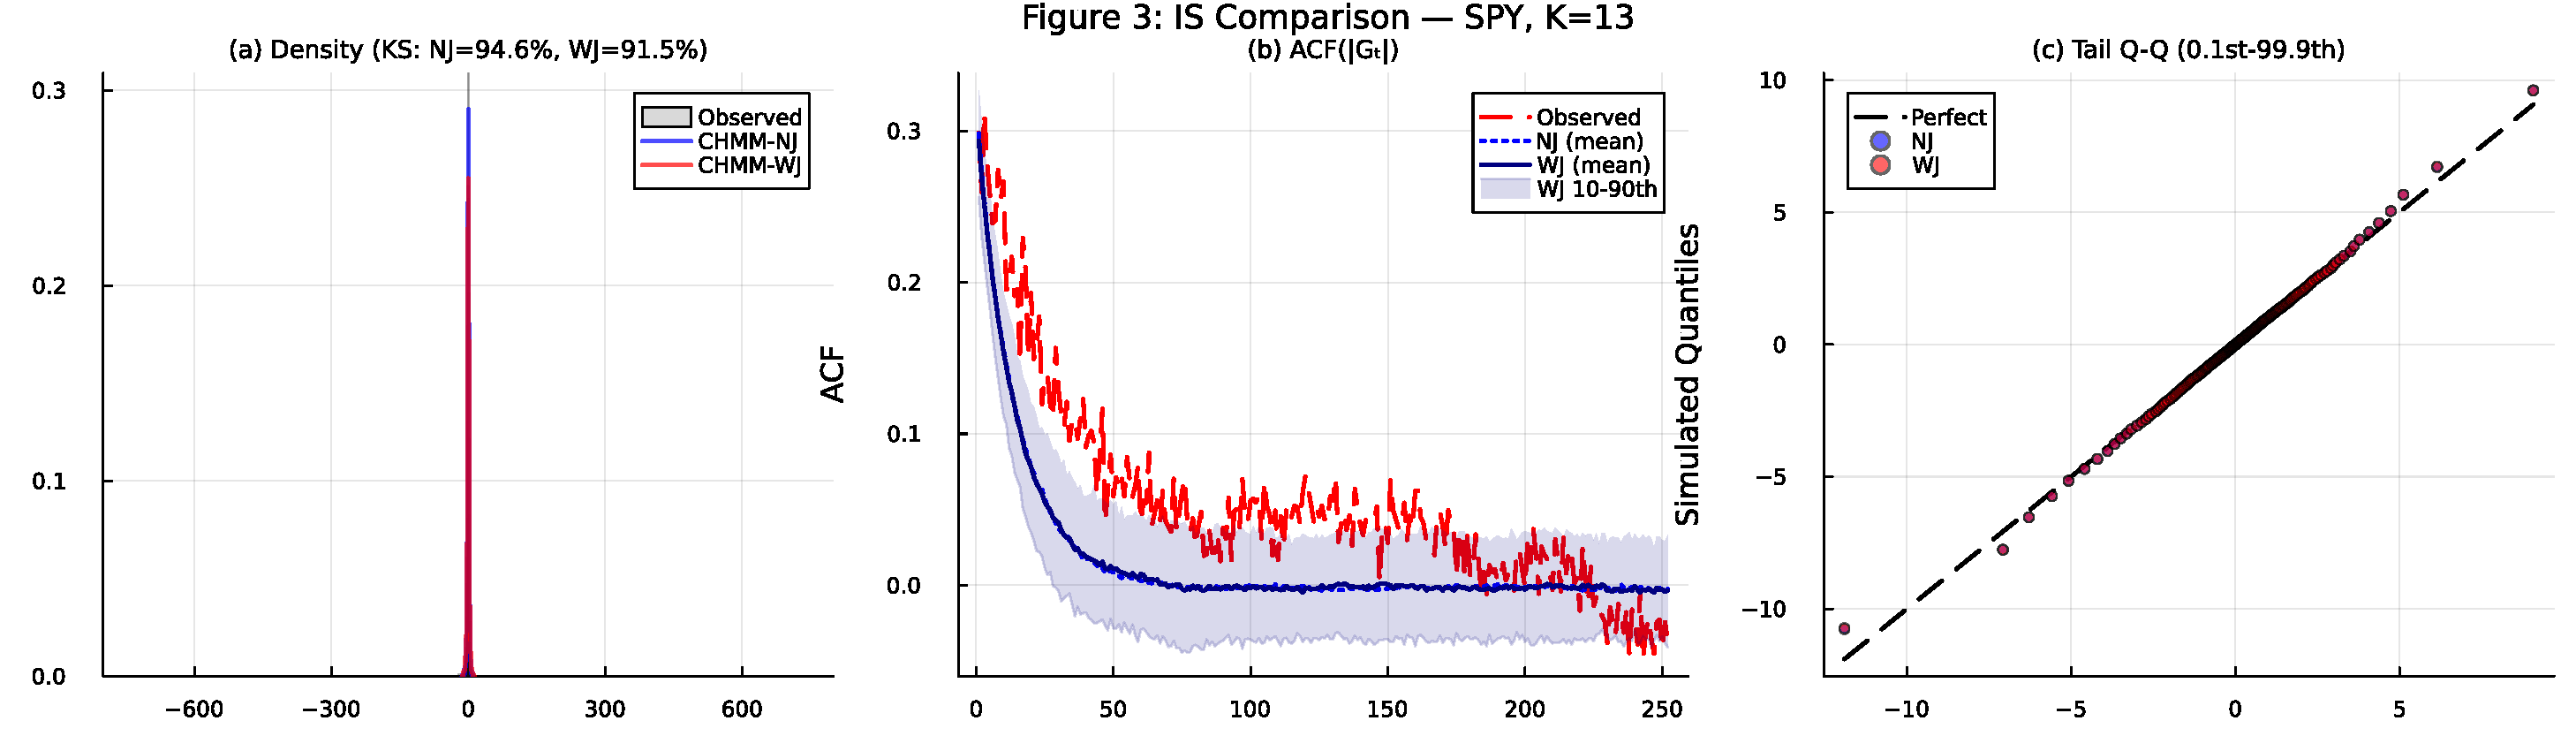
\includegraphics[width=\textwidth]{sections/figs/Fig-3-IS-Comparison-K13.pdf}
    \caption{$K = 13$}
    \label{fig:is_k13}
\end{subfigure}
\caption{In-sample model comparison at $K = 3, 6, 9, 13$. At all resolutions, the CHMM's simulated density matches the observed distribution and the ACF of absolute returns reproduces the slow decay pattern.}
\label{fig:is_all_k}
\end{figure}

\subsection{Out-of-Sample Comparison at All State Resolutions}

Figures~\ref{fig:oos_k3}--\ref{fig:oos_k13} show the out-of-sample validation panels for $K = 3, 6, 9$, and $13$.

\begin{figure}[H]
\centering
\begin{subfigure}[b]{0.48\textwidth}
    
\includegraphics[width=\textwidth]{sections/figs/Fig-4-OoS-Validation-K3.pdf}
    \caption{$K = 3$}
    \label{fig:oos_k3}
\end{subfigure}
\hfill
\begin{subfigure}[b]{0.48\textwidth}
    
\includegraphics[width=\textwidth]{sections/figs/Fig-4-OoS-Validation-K6.pdf}
    \caption{$K = 6$}
    \label{fig:oos_k6}
\end{subfigure}

\vspace{0.5cm}
\begin{subfigure}[b]{0.48\textwidth}
    
\includegraphics[width=\textwidth]{sections/figs/Fig-4-OoS-Validation-K9.pdf}
    \caption{$K = 9$}
    \label{fig:oos_k9}
\end{subfigure}
\hfill
\begin{subfigure}[b]{0.48\textwidth}
    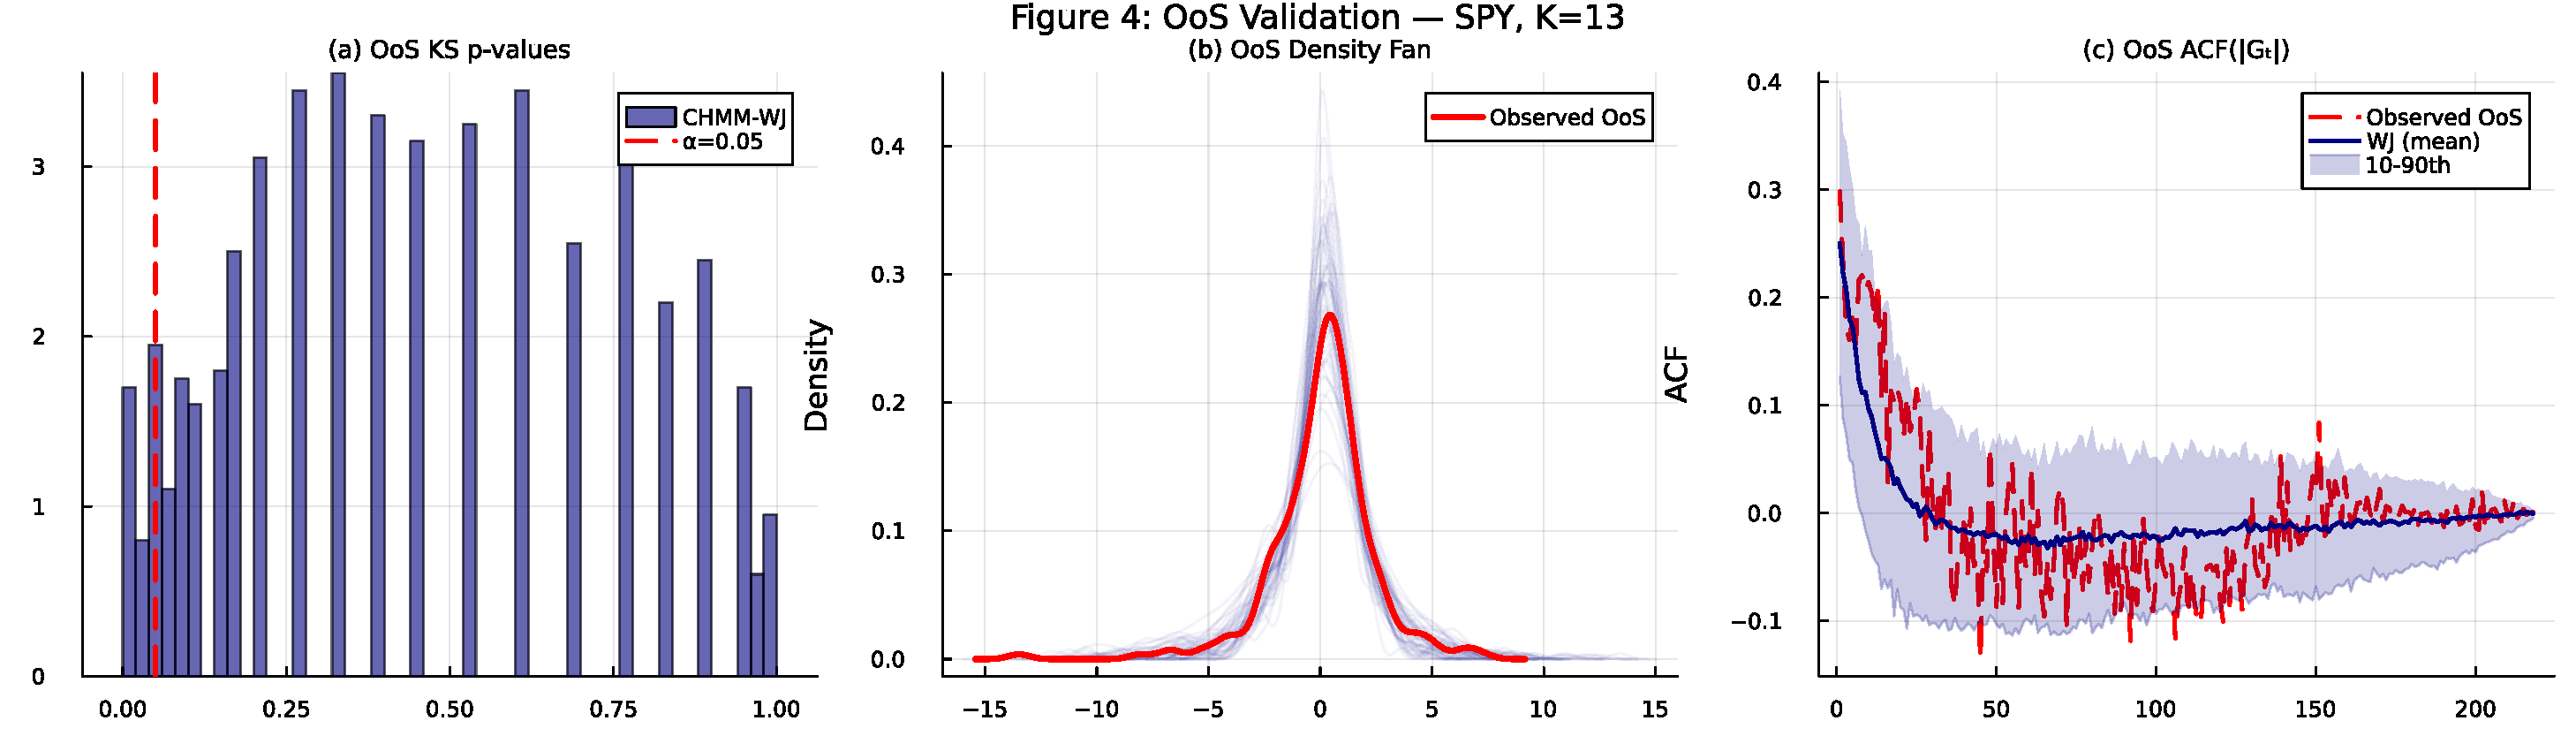
\includegraphics[width=\textwidth]{sections/figs/Fig-4-OoS-Validation-K13.pdf}
    \caption{$K = 13$}
    \label{fig:oos_k13}
\end{subfigure}
\caption{Out-of-sample validation at $K = 3, 6, 9, 13$. KS pass rates remain above 91\% at all resolutions, confirming robust generalization to the held-out 2025 data.}
\label{fig:oos_all_k}
\end{figure}

\subsection{Example Simulated Trajectories}

Figure~\ref{fig:trajectories} shows example simulated return trajectories for $K = 6$ and $K = 13$, illustrating the qualitative dynamics produced by the CHMM.
Both trajectories exhibit the characteristic pattern of financial returns: extended periods of low volatility punctuated by clusters of large-magnitude events.
The color coding indicates the hidden state at each time step, showing how regime transitions drive the alternation between calm and volatile periods.

\begin{figure}[H]
\centering
\begin{subfigure}[b]{0.48\textwidth}
    
\includegraphics[width=\textwidth]{sections/figs/Fig-Trajectory-Example-K6.pdf}
    \caption{$K = 6$}
\end{subfigure}
\hfill
\begin{subfigure}[b]{0.48\textwidth}
    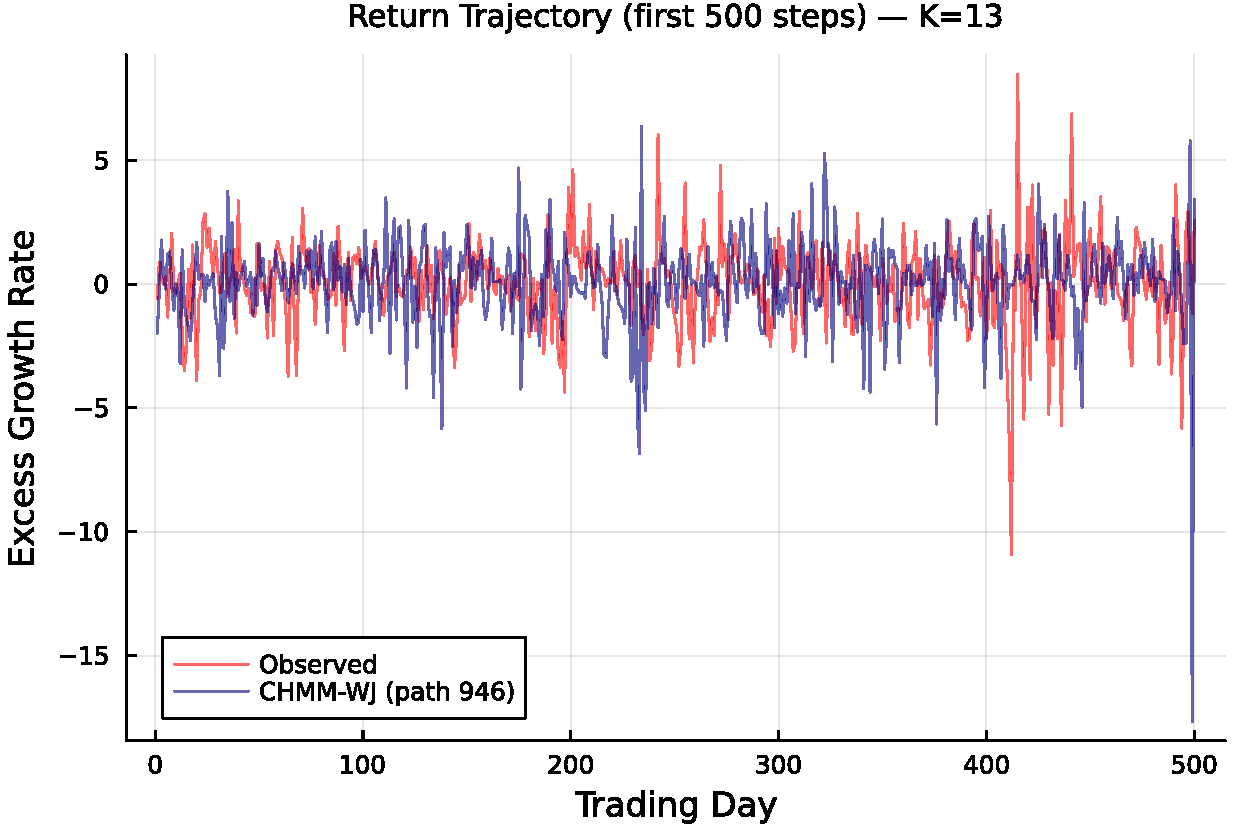
\includegraphics[width=\textwidth]{sections/figs/Fig-Trajectory-Example-K13.pdf}
    \caption{$K = 13$}
\end{subfigure}
\caption{Example simulated return trajectories for $K = 6$ and $K = 13$. Colors indicate the hidden state at each time step. The alternation between calm (central states) and volatile (tail states) periods produces the volatility clustering characteristic of empirical financial returns.}
\label{fig:trajectories}
\end{figure}

\subsection{VIX Results Detail}

The CHMM framework was applied to VIX daily log returns to test generalization beyond equity returns.
VIX returns exhibit positive skewness (reflecting asymmetric volatility spikes), pronounced mean reversion, and extreme excess kurtosis---properties that differ fundamentally from equity returns.

The CHMM captured these properties effectively: at higher state resolutions ($K \geq 9$), the model achieved IS KS pass rates above 99\%, demonstrating that the Gaussian mixture mechanism can approximate even the positively skewed, heavy-tailed marginal distribution of VIX returns.
The regime decomposition provided by the Viterbi algorithm aligned with known market events, assigning high-volatility states to crisis episodes and low-volatility states to calm market periods.

The VIX extension demonstrates that the CHMM framework is not limited to equity returns but applies more broadly to financial time series with regime-switching dynamics.
The decoded regimes and their associated median VIX levels provide the volatility map described in Section~\ref{sec:vix_methods}, linking the statistical model to the option pricing pathway.

\subsection{Algorithm Descriptions}
\label{sec:algorithms}

This section provides detailed pseudocode for all algorithms used in this study.
Algorithm~\ref{alg:baum_welch} describes the Baum-Welch (EM) procedure for learning CHMM parameters from continuous observations.
Algorithm~\ref{alg:viterbi} presents the Viterbi algorithm for decoding the most likely hidden state sequence.
Algorithm~\ref{alg:chmm_simulate} describes the CHMM simulation procedure for generating synthetic return paths.
Algorithm~\ref{alg:garch_fit} details the GARCH(1,1) fitting procedure via grid-initialized Nelder-Mead optimization.
Algorithm~\ref{alg:chmm_pricing} describes the regime-switching Monte Carlo option pricing pathway.
Algorithm~\ref{alg:implied_vol} presents the implied volatility inversion via bisection.

% ========================================================================================= %
% Algorithm 1: Baum-Welch (EM) for Continuous Gaussian HMM
% ========================================================================================= %
\begin{algorithm}[tp]
\caption{Baum-Welch (EM) algorithm for continuous Gaussian HMM parameter estimation}
\label{alg:baum_welch}
\small
\begin{algorithmic}[1]
\REQUIRE Observations $O_{1:T}$, Number of states $K$, Tolerance $\text{tol}$, Max iterations $\texttt{max\_iter}$
\ENSURE Transition matrix $\mathbf{T}$, Emission parameters $\{\mu_k, \sigma_k\}_{k=1}^K$, Initial distribution $\boldsymbol{\pi}$, Log-likelihood history

\STATE \textbf{--- Quantile-Based Initialization ---}
\STATE Sort observations: $O^{(\text{sort})} \leftarrow \text{sort}(O_{1:T})$.
\STATE Partition $O^{(\text{sort})}$ into $K$ equal-sized chunks $\{C_1, \ldots, C_K\}$.
\FOR{$k = 1$ to $K$}
    \STATE $\mu_k \leftarrow \text{mean}(C_k)$, \quad $\sigma_k \leftarrow \max(\text{std}(C_k),\; 10^{-6})$.
\ENDFOR
\STATE $T_{ij} \leftarrow 1/K$ for all $i, j$; \quad $\pi_k \leftarrow 1/K$ for all $k$.
\STATE $\mathcal{L}_{\text{prev}} \leftarrow -\infty$.

\STATE \textbf{--- EM Loop ---}
\FOR{$n = 1$ to $\texttt{max\_iter}$}

    \STATE \textbf{E-Step:} Compute emission log-likelihoods $\log B_{t,k} = \log \mathcal{N}(O_t \mid \mu_k, \sigma_k^2)$ for all $t, k$.

    \STATE \textit{Forward pass:}
    \STATE $\log \alpha_1(k) \leftarrow \log \pi_k + \log B_{1,k}$ for all $k$.
    \FOR{$t = 2$ to $T$}
        \FOR{$j = 1$ to $K$}
            \STATE $\log \alpha_t(j) \leftarrow \underset{i}{\text{logsumexp}}\!\left(\log \alpha_{t-1}(i) + \log T_{ij}\right) + \log B_{t,j}$
        \ENDFOR
    \ENDFOR

    \STATE \textit{Backward pass:}
    \STATE $\log \beta_T(k) \leftarrow 0$ for all $k$.
    \FOR{$t = T-1$ down to $1$}
        \FOR{$i = 1$ to $K$}
            \STATE $\log \beta_t(i) \leftarrow \underset{j}{\text{logsumexp}}\!\left(\log T_{ij} + \log B_{t+1,j} + \log \beta_{t+1}(j)\right)$
        \ENDFOR
    \ENDFOR

    \STATE \textit{Posterior quantities:}
    \FOR{$t = 1$ to $T$}
        \STATE $\gamma_t(k) \leftarrow \exp\!\left(\log \alpha_t(k) + \log \beta_t(k) - \underset{j}{\text{logsumexp}}(\log \alpha_t(j) + \log \beta_t(j))\right)$ for all $k$.
    \ENDFOR
    \FOR{$t = 1$ to $T-1$}
        \FOR{$i = 1$ to $K$}
            \FOR{$j = 1$ to $K$}
                \STATE $\xi_t(i,j) \leftarrow \exp\!\left(\log \alpha_t(i) + \log T_{ij} + \log B_{t+1,j} + \log \beta_{t+1}(j) - \text{norm}\right)$
            \ENDFOR
        \ENDFOR
    \ENDFOR

    \STATE \textbf{M-Step:} Re-estimate parameters.
    \STATE $\pi_k \leftarrow \gamma_1(k)$ for all $k$.
    \FOR{$k = 1$ to $K$}
        \STATE $\mu_k \leftarrow \sum_{t=1}^T \gamma_t(k) \cdot O_t \;/\; \sum_{t=1}^T \gamma_t(k)$
        \STATE $\sigma_k \leftarrow \max\!\left(\sqrt{\sum_{t=1}^T \gamma_t(k) \cdot (O_t - \mu_k)^2 \;/\; \sum_{t=1}^T \gamma_t(k)},\; 10^{-6}\right)$
    \ENDFOR
    \FOR{$i = 1$ to $K$}
        \STATE $T_{i,j} \leftarrow \sum_{t=1}^{T-1} \xi_t(i,j) \;/\; \sum_{t=1}^{T-1} \gamma_t(i)$ for all $j$.
    \ENDFOR

    \STATE \textbf{Convergence check:}
    \STATE $\mathcal{L}^{(n)} \leftarrow \underset{k}{\text{logsumexp}}(\log \alpha_T(k))$.
    \IF{$|\mathcal{L}^{(n)} - \mathcal{L}_{\text{prev}}| < \text{tol}$}
        \STATE \textbf{break}
    \ENDIF
    \STATE $\mathcal{L}_{\text{prev}} \leftarrow \mathcal{L}^{(n)}$.
\ENDFOR

\RETURN $\mathbf{T}, \{\mu_k, \sigma_k\}_{k=1}^K, \boldsymbol{\pi}$
\end{algorithmic}
\end{algorithm}

% ========================================================================================= %
% Algorithm 2: Viterbi Decoding
% ========================================================================================= %
\begin{algorithm}[tp]
\caption{Viterbi decoding for the most likely hidden state sequence}
\label{alg:viterbi}
\small
\begin{algorithmic}[1]
\REQUIRE Observations $O_{1:T}$, Trained CHMM $\mathcal{M} = (\mathbf{T}, \{\mu_k, \sigma_k\}, \boldsymbol{\pi})$
\ENSURE Most probable state sequence $S_{1:T}^*$

\STATE \textbf{--- Initialization ---}
\FOR{$k = 1$ to $K$}
    \STATE $\log \delta_1(k) \leftarrow \log(1/K) + \log \mathcal{N}(O_1 \mid \mu_k, \sigma_k^2)$.
\ENDFOR

\STATE \textbf{--- Forward Recursion ---}
\FOR{$t = 2$ to $T$}
    \FOR{$j = 1$ to $K$}
        \STATE $\text{vals}(i) \leftarrow \log \delta_{t-1}(i) + \log T_{ij}$ for all $i$.
        \STATE $\log \delta_t(j) \leftarrow \max_i \text{vals}(i) + \log \mathcal{N}(O_t \mid \mu_j, \sigma_j^2)$.
        \STATE $\psi_t(j) \leftarrow \arg\max_i \text{vals}(i)$.
    \ENDFOR
\ENDFOR

\STATE \textbf{--- Backtracking ---}
\STATE $S_T^* \leftarrow \arg\max_k \log \delta_T(k)$.
\FOR{$t = T-1$ down to $1$}
    \STATE $S_t^* \leftarrow \psi_{t+1}(S_{t+1}^*)$.
\ENDFOR

\RETURN $S_{1:T}^*$
\end{algorithmic}
\end{algorithm}

% ========================================================================================= %
% Algorithm 3: CHMM Simulation
% ========================================================================================= %
\begin{algorithm}[tp]
\caption{CHMM simulation of synthetic excess growth rate paths}
\label{alg:chmm_simulate}
\small
\begin{algorithmic}[1]
\REQUIRE Trained CHMM $\mathcal{M} = (\mathbf{T}, \{\mu_k, \sigma_k\}, \boldsymbol{\pi})$, Number of steps $M$, Number of paths $P$
\ENSURE Simulated return paths $\{\hat{G}^{(p)}_{1:M}\}_{p=1}^{P}$

\FOR{$p = 1$ to $P$}
    \STATE Sample initial state $S_1 \sim \text{Categorical}(\boldsymbol{\pi})$.
    \FOR{$t = 1$ to $M$}
        \STATE Emit observation $\hat{G}_t^{(p)} \sim \mathcal{N}(\mu_{S_t}, \sigma_{S_t}^2)$.
        \IF{$t < M$}
            \STATE Transition to next state $S_{t+1} \sim \text{Categorical}(\mathbf{T}_{S_t, \cdot})$.
        \ENDIF
    \ENDFOR
\ENDFOR

\RETURN $\{\hat{G}^{(p)}_{1:M}\}_{p=1}^{P}$
\end{algorithmic}
\end{algorithm}

% ========================================================================================= %
% Algorithm 4: GARCH(1,1) MLE via Grid-Initialized Nelder-Mead
% ========================================================================================= %
\begin{algorithm}[tp]
\caption{GARCH(1,1) maximum likelihood estimation via grid-initialized Nelder-Mead}
\label{alg:garch_fit}
\small
\begin{algorithmic}[1]
\REQUIRE Observations $G_{1:T}$
\ENSURE Fitted parameters $(\omega^*, \alpha^*, \beta^*, \mu^*)$, Conditional variance history $\sigma^2_{1:T}$

\STATE \textbf{--- Grid Search Initialization ---}
\STATE Set $\mu_{\text{init}} \leftarrow \text{mean}(G_{1:T})$, \quad $\hat{\sigma}^2 \leftarrow \text{var}(G_{1:T})$.
\STATE Define grids: $\alpha \in \{0.02, 0.05, 0.10, 0.15\}$, \quad $\beta \in \{0.70, 0.80, 0.85, 0.90\}$.
\STATE $\text{NLL}_{\min} \leftarrow \infty$.
\FOR{each $(\alpha, \beta)$ with $\alpha + \beta < 0.999$}
    \STATE $\omega \leftarrow \hat{\sigma}^2 (1 - \alpha - \beta)$.
    \STATE Evaluate $\text{NLL}(\omega, \alpha, \beta, \mu_{\text{init}})$:
    \STATE \quad $\sigma_1^2 \leftarrow \omega / (1 - \alpha - \beta)$.
    \FOR{$t = 1$ to $T$}
        \STATE $\text{NLL} \mathrel{-}= -\tfrac{1}{2}\left[\log(2\pi) + \log(\sigma_t^2) + (G_t - \mu)^2 / \sigma_t^2\right]$
        \IF{$t < T$}
            \STATE $\sigma_{t+1}^2 \leftarrow \omega + \alpha (G_t - \mu)^2 + \beta \sigma_t^2$
        \ENDIF
    \ENDFOR
    \IF{$\text{NLL} < \text{NLL}_{\min}$}
        \STATE $\text{NLL}_{\min} \leftarrow \text{NLL}$; \quad store $(\omega, \alpha, \beta, \mu_{\text{init}})$ as best.
    \ENDIF
\ENDFOR

\STATE \textbf{--- Nelder-Mead Optimization ---}
\STATE Initialize simplex from best grid point with 20\% perturbation per dimension.
\FOR{$\text{iter} = 1$ to $2000$}
    \STATE Evaluate NLL at all simplex vertices; sort by ascending NLL.
    \IF{$|\text{NLL}_{\text{worst}} - \text{NLL}_{\text{best}}| < 10^{-8}$}
        \STATE \textbf{break} \COMMENT{Converged}
    \ENDIF
    \STATE Compute centroid of all vertices except worst.
    \STATE \textit{Reflection:} $\mathbf{x}_r \leftarrow \mathbf{c} + (\mathbf{c} - \mathbf{x}_{\text{worst}})$.
    \IF{$f(\mathbf{x}_r) < f(\mathbf{x}_{\text{best}})$}
        \STATE \textit{Expansion:} $\mathbf{x}_e \leftarrow \mathbf{c} + 2(\mathbf{x}_r - \mathbf{c})$. Replace worst with better of $\mathbf{x}_r, \mathbf{x}_e$.
    \ELSIF{$f(\mathbf{x}_r) < f(\mathbf{x}_{\text{2nd worst}})$}
        \STATE Replace worst with $\mathbf{x}_r$.
    \ELSE
        \STATE \textit{Contraction:} $\mathbf{x}_c \leftarrow \mathbf{c} + 0.5(\mathbf{x}_{\text{worst}} - \mathbf{c})$.
        \IF{$f(\mathbf{x}_c) < f(\mathbf{x}_{\text{worst}})$}
            \STATE Replace worst with $\mathbf{x}_c$.
        \ELSE
            \STATE \textit{Shrink:} $\mathbf{x}_i \leftarrow \mathbf{x}_{\text{best}} + 0.5(\mathbf{x}_i - \mathbf{x}_{\text{best}})$ for all $i \neq \text{best}$.
        \ENDIF
    \ENDIF
\ENDFOR

\STATE \textbf{--- Variance Reconstruction ---}
\STATE Extract $(\omega^*, \alpha^*, \beta^*, \mu^*)$ from best vertex.
\STATE $\sigma_1^2 \leftarrow \omega^* / (1 - \alpha^* - \beta^*)$.
\FOR{$t = 2$ to $T$}
    \STATE $\sigma_t^2 \leftarrow \omega^* + \alpha^* (G_{t-1} - \mu^*)^2 + \beta^* \sigma_{t-1}^2$.
\ENDFOR

\RETURN $(\omega^*, \alpha^*, \beta^*, \mu^*)$, $\sigma^2_{1:T}$
\end{algorithmic}
\end{algorithm}

% ========================================================================================= %
% Algorithm 5: CHMM Regime-Switching Monte Carlo Option Pricing
% ========================================================================================= %
\begin{algorithm}[tp]
\caption{CHMM regime-switching Monte Carlo option pricing}
\label{alg:chmm_pricing}
\small
\begin{algorithmic}[1]
\REQUIRE Trained CHMM $\mathcal{M}$ on VIX returns, VIX price series, Contract $(S_0, K, T, r)$, Number of paths $P$
\ENSURE Option price $\hat{C}$ (or $\hat{P}$), Standard error

\STATE \textbf{--- Volatility Map Construction ---}
\STATE Decode VIX state sequence: $S_{1:T}^* \leftarrow \text{Viterbi}(O_{1:T}^{\text{VIX}}, \mathcal{M})$.
\FOR{$k = 1$ to $K$}
    \STATE $\bar{V}_k \leftarrow \text{median}(\{\text{VIX}_t : S_t^* = k\}) \;/\; 100$ \COMMENT{Map state to equity volatility}
\ENDFOR

\STATE \textbf{--- Stationary Distribution ---}
\STATE Compute $\bar{\boldsymbol{\pi}} = \lim_{n \to \infty} \boldsymbol{\pi} \mathbf{T}^n$ via matrix power iteration.

\STATE \textbf{--- Monte Carlo Simulation ---}
\STATE Set $n_{\text{steps}} \leftarrow \lceil T \times 252 \rceil$, \quad $\Delta t \leftarrow T / n_{\text{steps}}$.
\FOR{$p = 1$ to $P$}
    \STATE Sample initial state $s_0 \sim \text{Categorical}(\bar{\boldsymbol{\pi}})$.
    \STATE Simulate state path: $(S_1, \ldots, S_{n_{\text{steps}}}) \leftarrow \mathcal{M}(s_0,\; n_{\text{steps}})$.
    \STATE $S \leftarrow S_0$.
    \FOR{$t = 1$ to $n_{\text{steps}}$}
        \STATE $\sigma_t \leftarrow \bar{V}_{S_t}$.
        \STATE $Z \sim \mathcal{N}(0,1)$.
        \STATE $S \leftarrow S \cdot \exp\!\left((r - \sigma_t^2 / 2)\Delta t + \sigma_t \sqrt{\Delta t}\; Z\right)$.
    \ENDFOR
    \STATE $\text{payoff}_p \leftarrow \max(S - K, 0)$ for calls, or $\max(K - S, 0)$ for puts.
\ENDFOR

\STATE $\hat{C} \leftarrow e^{-rT} \cdot \frac{1}{P}\sum_{p=1}^{P} \text{payoff}_p$.
\STATE $\text{SE} \leftarrow \text{std}(e^{-rT} \cdot \text{payoffs}) \;/\; \sqrt{P}$.

\RETURN $\hat{C}$, SE
\end{algorithmic}
\end{algorithm}

% ========================================================================================= %
% Algorithm 6: Implied Volatility Inversion via Bisection
% ========================================================================================= %
\begin{algorithm}[tp]
\caption{Implied volatility inversion via bisection}
\label{alg:implied_vol}
\small
\begin{algorithmic}[1]
\REQUIRE Contract $(S_0, K, T, r)$, Market price $V_{\text{mkt}}$, Tolerance $\text{tol}$, Max iterations $N_{\max}$
\ENSURE Implied volatility $\sigma_{\text{IV}}$

\STATE $\sigma_{\text{lo}} \leftarrow 10^{-4}$, \quad $\sigma_{\text{hi}} \leftarrow 5.0$.
\FOR{$n = 1$ to $N_{\max}$}
    \STATE $\sigma_{\text{mid}} \leftarrow (\sigma_{\text{lo}} + \sigma_{\text{hi}}) / 2$.
    \STATE $V_{\text{BS}} \leftarrow \text{BlackScholes}(S_0, K, T, r, \sigma_{\text{mid}})$.
    \STATE $\text{err} \leftarrow V_{\text{BS}} - V_{\text{mkt}}$.
    \IF{$|\text{err}| < \text{tol}$}
        \RETURN $\sigma_{\text{mid}}$
    \ELSIF{$\text{err} > 0$}
        \STATE $\sigma_{\text{hi}} \leftarrow \sigma_{\text{mid}}$.
    \ELSE
        \STATE $\sigma_{\text{lo}} \leftarrow \sigma_{\text{mid}}$.
    \ENDIF
\ENDFOR

\RETURN $(\sigma_{\text{lo}} + \sigma_{\text{hi}}) / 2$
\end{algorithmic}
\end{algorithm}


\end{document}
